\documentclass[conference,harvard,brazil]{sbatex}

\usepackage[latin1]{inputenc}
%\usepackage[brazil]{babel}
%\usepackage[T1]{fontenc}
\usepackage{ae}

\makeatletter
\def\verbatim@font{\normalfont\ttfamily\footnotesize}
\makeatother

\usepackage{graphics} % for pdf, bitmapped graphics files
\usepackage{epsfig} % for postscript graphics files
%\usepackage{mathptmx} % assumes new font selection scheme installed
%\usepackage{times} % assumes new font selection scheme installed
\usepackage{amsmath}
\usepackage{amssymb}  % assumes amsmath package installed
%\let\proof\relax
%\let\endproof\relax
%\usepackage{amsthm}
\usepackage{color}
%\usepackage{mathtools}
\usepackage{tabularx} %used to chose the widht of tables
\usepackage{multirow}
\usepackage{epstopdf}
\let\labelindent\relax
\usepackage[inline]{enumitem}

\newtheorem{remark}{Coment�rio}
\theoremstyle{plain}
\newtheorem{definition}{Defini��o}
\newtheorem{teorema}{Teorema}
\newtheorem{algorithm}{Algoritmo}
\newcommand{\sref}[1]{Se��o~\ref{#1}}
\newcommand{\fref}[1]{Fig.~\ref{#1}}
\newcommand{\tref}[1]{Tabela~\ref{#1}}
\newcommand{\norm}[1]{\left\lVert#1\right\rVert}
\newcommand{\aref}[1]{Suposi��o~\ref{#1}}
\newcommand{\algref}[1]{\textbf{Algoritmo~\ref{#1}}}
%\renewcommand{\qedsymbol}{}
\newcommand{\rev}[1]{{\color{red}#1}}
\newcommand{\mat}[1]{\begin{bmatrix}#1\end{bmatrix}}

\begin{document}
\thispagestyle{plain}
\pagestyle{plain}

\title{Identifica��o e Controle por Torque Computado de uma Plataforma Inercial para Estabiliza��o e Rastreamento da Linha de Visada}

%%%%%%%%%%%%%%%%%%%%%%%%%%%%%%%%%%%%%%%%%%%%%%%%%%%%%%%%%%%%%
%
% O processo de revisao do CBA 2014 sera DOUBLE BLIND, portanto NAO inclua
% autores na vers�o que ser� submetida para revis�o
%
%%%%%%%%%%%%%%%%%%%%%%%%%%%%%%%%%%%%%%%%%%%%%%%%%%%%%%%%%%%%%
%
\author{Matheus F. Reis, Jo�o C. Monteiro, Guilherme P. S. Carvalho, Alex F. Neves, Alessandro J. Peixoto}
{matheus.ferreira.reis@gmail.com, jcmonteiro@poli.ufrj.br, guilherme.ps.carvalho@gmail.com, alexfneves@gmail.com, jacoud@coep.ufrj.br}
\address{COPPE/UFRJ\\ Ilha do Fund�o, Rio de Janeiro, RJ, Brasil}
%
%\author{Jo�o C. Monteiro}{jcmonteiro@poli.ufrj.br}
%\address{Endere�o do Jo�o\\ Em algum lugar\\ Rio de Janeiro, RJ, Brasil}
%
%\author{Guilherme P. S. Carvalho}{guilherme.ps.carvalho@gmail.com}
%\address{Endere�o do Zeca\\ Em algum lugar\\ Rio de Janeiro, RJ, Brasil}
%
%\author{Alex F. Neves}{alexfneves@gmail.com}
%\address{Endere�o do Alex\\ Em algum lugar\\ Rio de Janeiro, RJ, Brasil}
%
%\author{Alessandro J. Peixoto}{jacoud@coep.ufrj.br}
%\address{Endere�o do Jacoud\\ Em algum lugar\\ Rio de Janeiro, RJ, Brasil}

%% Abstract section
\twocolumn[
\maketitle
%\selectlanguage{english}

\begin{abstract}
The majority of works in line of sight (LOS) stabilization and tracking using inertially stabilized platforms (ISP) apply simple linear controllers to achieve the required performance. Commonly, linear models are employed to describe the relationship between torque and position of the ISP joints, such as a double integrator with an inertia gain.
%
However, high-accuracy and fast motion applications may require more complex control techniques, demanding accurate dynamic and kinematic models, and system \textit{identification} procedures.
%
In this work, we propose a cascade control topology for stabilization and tracking of the line of sight of a camera in a 3-DOF ISP installed on a vessel. Using measurements from joint encoders and an inertial navigation system (INS) fixed on the vessel, an inner controller cancels the \textit{dynamic} disturbances acting on the ISP joints, while an outer kinematic controller ensures LOS tracking.
%
For this type of controller, the ISP joint axes are critical parameters with respect to the tracking performance, since their uncertainty introduce bias in the control response. For this reason, a simple, yet efficient identification procedure for the joint axes is proposed.
%
Simulations in Gazebo using the Rock robotics framework and a Unity-based viewer show the efficiency of this procedure and the performance of the proposed cascade controller for LOS stabilization and tracking.
\end{abstract}

\keywords{Line of sight stabilization, inertial platform, computed torque control.}
%%%%%%%%%%%%%%%%%%%%%%%%%%%%
\selectlanguage{brazil}

\begin{abstract}
A maioria dos trabalhos em estabiliza��o e rastreamento da linha de visada (LOS) com plataformas inerciais (ISPs) utilizam simples controladores lineares para atingir o n�vel de performance exigido. Geralmente, modelos lineares s�o suficientes para descrever a rela��o �ngulo-torque para as juntas da plataforma, tais como um simples duplo integrador.
%
Por�m, em opera��es que requerem alta velocidade e/ou acur�cia, t�cnicas de controle mais complexas podem ser necess�rias. Tais t�cnicas em geral demandam modelos mais realistas para o sistema considerado, bem como procedimentos para a identifica��o de par�metros destes modelos.
%
Neste trabalho, � proposta uma topologia de controle em cascata para estabiliza��o e rastreamento da linha de visada de uma c�mera, utilizando uma plataforma inercial de 3 eixos instalada em um navio.
%
Utilizando medi��es de encoders localizados nas juntas e um sistema de navega��o inercial (INS) acoplado ao navio, um controlador interno cancela perturba��es din�micas devido ao movimento do navio, enquanto um controlador cinem�tico externo garante o rastreamento da LOS.
%
Neste abordagem, os eixos das juntas s�o par�metros cr�ticos em rela��o ao desempenho de rastreamento, pois sua incerteza introduz um bias em rela��o a refer�ncia desejada.
%
Por isso, um simples e eficiente procedimento de identifica��o � proposto.
%
Simula��es em Gazebo com o ambiente de simula��o Rock e um visualizador baseado em Unity mostram a efici�ncia do procedimento e o desempenho do controlador proposto.
\end{abstract}

\keywords{Estabiliza��o da linha de visada, plataformas inerciais, controle por torque computado.}
]
\selectlanguage{brazil}
%%%%%%%%%%%%%%%%%%%%%%%%%%%%%%%%%%%%%%%%%%%%%%%%%%%%%%%%%%%%%%%%%%%%%%%%%%%%%%%%
%%%%%%%%%%%%%%%%%%%%%%%%%%%%%%%%%%%%%%%%%%%%%%%%%%%%%
\section{Introdu��o}
\label{sec:intro}

%Line of sight (LOS) stabilization is a common and challenging problem in the
%control literature. Inertially stabilized platforms (ISP) are widely used for 
%payload stabilization and tracking applications, when a sensor must accurately 
%point to a target in a dynamic environment.
%
Estabiliza��o da linha de visada (LOS) � um problema comum na literatura de controle.
Plataformas inerciais (do ingl�s {\it Inertial Stabilization Platform} - ISP) s�o utilizadas para estabiliza��o de cargas em aplica��es de estabiliza��o e rastreamento, quando um sensor precisa ser estabilizado e/ou apontado de forma precisa em um ambiente din�mico.
%
%Some examples are cameras for aerial surveying and entertainment industry 
%\cite{Hurak2009}, long-range sensors on vehicles \cite{Debruin2008}, military applications \cite{Kazemy2007} and thermal cameras for oil spill 
%detection \cite{skjelten2011ship}.
%
Alguns exemplos s�o: c�meras para vigil�ncia a�rea e para a ind�stria de entretenimento \cite{Hurak2009}, sensores de longo alcance para ve�culos \cite{Debruin2008}, aplica��es militares \cite{Kazemy2007} e c�meras t�rmicas para detec��o de vazamento de �leo \cite{skjelten2011ship}.

%%% Direct VS Indirect Stabilization %%%
%ISPs are usually gimbaled structures mounted on a 
%mobile base (vehicle) with motors equipped with encoders/tachometers 
%and a payload fixed on the last gimbal. Gyroscopes 
%or inertial navigation systems (INS) are employed to close the control loop by 
%either measuring the vehicle motion (\textit{indirect stabilization}) or 
%directly measuring the payload motion (\textit{direct stabilization}) 
%\cite{Kennedy2003}.
%
ISPs s�o geralmente compostas por gimbals conc�ntricos montados em uma base m�vel (ve�culo) equipadas com motores e encoders/tac�metros com uma carga fixa no �ltimo gimbal.
%
Girosc�pios ou sistemas de navega��o inercial (do ingl�s {\it Inertial Navigation System} - INS) s�o usados para medir o movimento do ve�culo (\textit{estabiliza��o indireta}) ou medir diretamente o movimento da carga (\textit{estabiliza��o indireta}).

%Typically, it is not possible to use state-of-the-art inertial sensor 
%technology in a direct configuration, due to weight and size limitations, which are irrelevant for the indirect method, specially for applications in large vehicles, such as a ship.
%%
%For the indirect method, the estimation of the payload motion from the vehicle motion and joint encoders measurements is required and may be affected by several sources of errors, such as ISP geometric uncertainty, encoder precision and stiffness of the gimbals \cite{Kennedy2003}.
%%
%Naturally, these errors may lead to unsatisfactory performance when applying 
%model-based controllers for LOS stabilization and tracking.
%
Tipicamente, n�o � poss�vel utilizar sensores de �ltima gera��o em configura��o direta devido � limita��es de tamanho e carga da ISP.
%
Em geral, tais limita��es inexistem na configura��o indireta, especialmente em aplica��es com grandes ve�culos, como navios. 
%
Por�m, neste m�todo � necess�rio realizar a estima��o do movimento da carga a partir do movimento medido do ve�culo e da ISP. Esta estimativa ser� afetada por diversas fontes de erros, como incerteza param�trica, precis�o dos encoders e rigidez da estrutura mec�nica da plataforma, o que pode resultar em n�veis de performance insuficientes ao se utilizar controladores baseados na lineariza��o do modelo do sistema \cite{Kennedy2003}.

%To ensure satisfactory control performance and develop trustworthy models
%of real robotic systems, a precise knowledge of the geometric and dynamic parameters of the system is required.
%%
%Geometric parameters ($\Pi_g$) influence the ISP Jacobian matrix and are composed of the joint axes vectors and the distances between joints.
%%
%Dynamic parameters ($\Pi_d$) influence the mass, Coriolis, and gravity matrices
%and are composed each link mass, inertia and center of mass position.
%
Para garantir resultados satisfat�rios e desenvolver modelos confi�veis para o sistema real, � necess�rio um conhecimento preciso dos par�metros do sistema.
%
Par�metros geom�tricos ($\Pi_g$) influenciam o Jacobiano da ISP e consistem nas componentes dos vectores de eixo e dist�ncias entre as juntas.
%
Par�metros din�micos ($\Pi_d$) influenciam as matrizes de massa, Coriolis e os termos de gravidade da equa��o din�mica, e s�o compostos por massas, componentes de in�rcia e posi��o dos centros de massa dos elos.

%Parameter identification consists in modeling, design of sufficiently rich
%trajectories, data acquisition and processing, parameter estimation and model
%validation.
%%
%Most of the ongoing research on parameter identification is devoted to the
%estimation of dynamic parameters.
%%
%In~\cite{Swevers2007dynamic,Calanca2011mimo}, finite Fourier series are used to
%generate trajectories capable of exciting every parameter, while identification
%is based on weighted least-squares.
%%
%In~\cite{Wu2012closed}, trajectories are generated using modified Fourier series
%and the identification is based on a maximum likelihood approach.
%%
%Recently, an algorithm based on linear matrix inequalities (LMIs) with
%trajectories generated by finite Fourier series was proposed to identify the dynamic parameters of the da Vinci research kit robotic arms~\cite{Fontanelli2017modelling}.
%%
%This approach also guarantees the physical feasibility of the identified
%parameters, a property that is not considered in least-squares and likelihood
%methods.
%
%A {\it identifica��o de par�metros} consiste na modelagem, projeto de trajet�rias suficientemente ricas, aquisi��o de dados e processamento, estima��o param�trica e valida��o de modelos.
%
Grande parte da pesquisa atual em {\it identifica��o param�trica} est� voltada para a estima��o dos par�metros din�micos.
%
Em~\cite{Swevers2007dynamic,Calanca2011mimo}, s�ries de Fourier finitas s�o utilizadas para gera��o de trajet�rias suficientemente ricas para excitar cada par�metro, e a identifica��o � baseada no m�todo dos m�nimos quadrados.
%
Em~\cite{Wu2012closed}, as trajet�rias s�o geradas utilizando s�ries de Fourier modificadas e a identifica��o � baseada no m�todo de maximiza��o da verossimilhan�a (maximum likelihood).
%
Recentemente, um algoritmo baseado em desigualdades lineares matriciais (LMIs) com trajet�rias geradas por s�ries de Fourier finitas foi proposto para identificar os par�metros din�micos para o kit de rob�tica cir�rgica {\it da Vinci}~\cite{Fontanelli2017modelling}.
%
Este m�todo tamb�m garante a viabilidade f�sica dos par�metros identificados, propriedade que n�o � considerada nos m�todos anteriores.

%In contrast to these works, we focus on the identification of geometric parameters.
%%
%Although important, the impact in system performance due to the uncertainty of
%dynamic parameters can usually be mitigated by an appropriate choice of control
%architecture and control tuning.
%%
%In~\cite{Reis2018}, it is shown that even in the presence of large parameter
%uncertainties, a Computed Torque plus PID (CTPID) controller guarantees satisfactory performance.
%%
%On the other hand, uncertainty in geometric parameters can lead to great amount of bias in the tracking performance.
%
Em contraste com tais trabalhos, focamos na identifica��o dos par�metros geom�tricos. Apesar de importante, o impacto na performance devido � incerteza nos par�metros din�micos normalmente pode ser reduzida por uma escolha apropriada da arquitetura e por uma boa sintonia do controlador.
%
Em~\cite{Reis2018}, mostra-se que mesmo sob consider�veis incertezas param�tricas, um controlador por torque computado com PID garante um desempenho satisfat�rio.
%
Por outro lado, a incerteza nos par�metros geom�tricos pode causar grandes n�veis de bias.

%In this work, we propose an identification procedure for the joint axes vectors and an indirect stabilization cascade control topology. The inner loop is a computed torque control in joint space to compensate the platform nonlinear dynamics, reducing the joint dynamics to a disturbed double integrator.
%%
%The outer loop attempts to cancel further kinematic disturbances and a PID controller in operational space ensures LOS tracking.
%%
%This control architecture is robust to parameter uncertainties and it differs
%from the one proposed in~\cite{Reis2018}, providing a simpler and more
%complete robustness analysis with respect to parameter uncertainty.
%%
%Simulations in Gazebo using the Rock robotics framework and a customized user interface based on Unity show the robustness and effectiveness of the proposed control and the identification algorithm, which is able to accurately find the joint axes even in the presence of large measurement noise.
%
Neste trabalho, propomos um m�todo de identifica��o para os vetores de eixos das juntas e uma topologia de controle em cascata para estabiliza��o e rastreamento. A malha de controle interna � um controlador por torque computado no espa�o das juntas, respons�vel por compensar a din�mica n�o-linear da planta, reduzindo-a a um duplo integrador com perturba��o.
%
A malha externa procura cancelar dist�rbios cinem�ticos e utiliza um controle PID no espa�o operacional para garantir o rastreamento.
%
Esta arquitetura � robusta a incertezas param�tricas e difere da proposta em~\cite{Reis2018} por fornecer uma an�lise mais simples e completa em rela��o � robustez do controle � incertezas param�tricas.
%
Simula��es em Gazebo utilizando o ambiente de simula��o Rock e uma interface de usu�rio baseada em Unity demonstram a robustez e performance do algoritmo de controle e do m�todo de identifica��o propostos.
 
%%%%%%%%%%%%%%%%%%%%%%%%%%%%%%%%%%%%%%%%%%%%%%%%%%%%%%%%%%%%%%%%%%%%%%%%%%%%%%%%%%%%%%%%%%%%%%%%%%%%%%%%
\section{Modelagem}
\label{sec:modeling}

%In this section, a procedure to derive the kinematic and dynamic models of an ISP fixed on a mobile base is given. 
%
%Nesta se��o, apresentamos o procedimento de c�lculo do modelo cinem�tico e din�mico de uma ISP fixa em uma base m�vel.

%%%%%%%%%%%%%%%%%%%%%%%%%%%%%%%%%%%%%%%%%%%%%%%%%%%%%%%%%%%%%%%%%%%%%%%%%%%%%%%%%%%%%%%%%%%%%%%%%%%%%%%%
\subsection{Nota��o e Conven��es}
\label{sec:definitions}

%This section presents the notations and definitions used in this work. Let $\mathbb{N}_0 = \{0,1,2,\dots\}$ and define $\mathbb{\bar{N}}_1 = \{ \bar{1}\,, \bar{2}\,, \hdots \}$. Unless otherwise stated, $i, j, k \in \mathbb{N}_0 \cup \mathbb{\bar{N}}_1 \cup \{\bar{b},b,s,c\}$.
%
Esta se��o introduz nota��es e defini��es utilizadas neste trabalho. Sejam os conjuntos $\mathbb{N}_0 = \{0,1,2,\dots\}$ e $\mathbb{\bar{N}}_1 = \{ \bar{1}\,, \bar{2}\,, \hdots \}$. A menos que seja dito o contr�rio,
$i, j, k \in \mathbb{N}_0 \cup \mathbb{\bar{N}}_1 \cup \{\bar{b},b,s,c\}$.
%
\begin{figure}[ht]
    \centering
    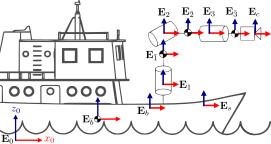
\includegraphics[width=.95\columnwidth]{figs/ship_conventions.pdf}
    \caption{Conven��es para os sistemas de refer�ncia da ISP de tr�s eixos.}
    \label{fig:HEADS_convention}
\end{figure}

%Considering \fref{fig:HEADS_convention}, define the following:
Considerando a \fref{fig:HEADS_convention}, defina o seguinte:
%
\begin{itemize}
\item $\mathbf{E}_{0}$: sistema inercial de refer�ncia;
%\item $\mathbf{E}_{s}$: INS frame, placed anywhere on the vehicle or on the last link for the indirect and direct stabilization configurations, respectively;
\item $\mathbf{E}_{\bar{i}}$: fixo no corpo $i$ com origem em seu centro de gravidade (CG) ($i \in \mathbb{N}_1 \cup \{b\}$);
\item $\mathbf{E}_{i}$: fixo no corpo $i$ com origem no eixo da $i$-n�sima junta $(i \in \mathbb{N}_1)$;
\item $\mathbf{E}_{s}$: fixo na INS em configura��o indireta;
\item $\mathbf{E}_{b}$: fixo no ve�culo ($\mathbf{E}_{b} \equiv \mathbf{E}_{s}$);
%We consider $\mathbf{E}_b \equiv \mathbf{E}_s$ (or $\mathbf{E}_b$ located on $\mathbf{E}_1$) for the indirect (or direct) configuration;
\item $\mathbf{E}_{c}$: fixo na c�mera, no �ltimo elo;
%\item $\mathbf{E}_{t}$: fixed on the target georeferenced position;
\item $R_{ij} \in SO(3)$: matriz de rota��o descrevendo a orienta��o de $\mathbf{E}_j$ em rela��o � $\mathbf{E}_i$;
%Of course, $R_{i,i} = I_{3}$, where $I_{3} \in \mathbb{R}^{3 \times 3}$ is the identity matrix;
%
\item $x^k_i\,,y^k_i\,,z^k_i \in \mathbb{R}^{3}$: vetores da base can�nica de $\mathbf{E}_i$, escritos em $\mathbf{E}_k$;
%
%\item $p_{0i} \in \mathbb{R}^{3}$: inertial position of the origin of frame $\mathbf{E}_i$;
%
\item $p^{k}_{ij} \in \mathbb{R}^{3}$: vetor de posi��o da origem de $\mathbf{E}_i$ at� a origem de $\mathbf{E}_{j}$, representado em $\mathbf{E}_k$;
%We use $r=p$ for position and $r=v$ for linear velocity, for example;
%
\item $v^{k}_{ij} \in \mathbb{R}^{3}$: velocidade linear de $\mathbf{E}_i$ em rela��o � $\mathbf{E}_{j}$, escrita em $\mathbf{E}_k$;
%
\item $\omega^{k}_{ij} \in \mathbb{R}^{3}$: velocidade angular de $\mathbf{E}_i$ em rela��o � $\mathbf{E}_{j}$, escrita em $\mathbf{E}_k$;
%
%\item $V^{k}_{ij} = [\, {v^{k}_{ij}}^{T} \,\,\, {\omega^{k}_{ij}}^{T} \,]^T \in \mathbb{R}^{6}$: velocity twist (linear and angular velocities) from $\mathbf{E}_i$ to  $\mathbf{E}_{j}$, written in $\mathbf{E}_k$;
%
\item $g_{ij} \in SE(3)$: transforma��o homog�nea de $\mathbf{E}_j$ at� $\mathbf{E}_i$;
%depending on $R_{ij}$ and on the position vector $p^i_{ij}$;
%
\item $h^{j}_{i} \in \mathbb{R}^{3}$: vetor unit�rio definindo o eixo de rota��o da $i$-n�sima junta, representado em $\mathbf{E}_j$ ($i \in \mathbb{N}_1$);
%
%\item $\omega_i \in \mathbb{R}^{3}$: angular velocity of body $i$ seen and represented in the inertial frame 					 $\mathbf{E}_0$ ($i \in \mathbb{N}_1 \cup \{b\}$). Mathematically, $\omega_i$ is defined as the twist coordinates of the $so(3)$ 			 Lie algebra as $\hat{\omega}_i = \dot{R}_i R^{T}_{i}$;

\item $m_i \in \mathbb{R} ,\, I^{i}_{i} \in \mathbb{R}^{3 \times 3}$: massa e tensor de in�rcia do corpo $i$ representado em $\mathbf{E}_{i}$ ($i \in \mathbb{N}_1 \cup \{b\}$);
%
%\item $\overline{I}^i_i =
%\left[\begin{array}{cc}
%\!\! m_i \, I_{3\times3} \!\!&\!\!  0 \!\! \\
%\!\! 0 \!\!&\!\! I^i_i \!\!
%\end{array}\right]$: augmented inertia matrix of body $i$;
%of body $i$ written in $\mathbf{E}_{i} (i \in \mathbb{N}_1 \cup \{b\})$.
%
\item $\mathbf{S} : \mathbb{R}^3 \mapsto \mathrm{so}(3)$ operador do produto vetorial;
%
\item $\mathbf{I}_{n} \in \mathbb{R}^{n \times n}$: matriz identidade de dimens�o $n$.
%
\end{itemize}
%
%\rev{Also, since the indirect stabilization approach is proposed, the INS frame is supposed to be $\mathbf{E}_{b}$}.
%
%Note that, by the definition of $\mathbf{E}_{i}$, $I^i_i$ is a constant matrix. If $\mathbf{E}_{i}$ is chosen to be aligned with the principal axis of inertia of rigid body $i$, $I^i_i$ is also diagonal.
%Therefore, for simplicity, it is supposed that the principal moments of the inertia matrix of body $i$ are known.
%%
%Also, in the case of a 3-DOF ISP, we suppose that $\mathbf{E}_{e} \equiv \mathbf{E}_{3}$.
%
%%%%%%%%%%%%%%%%%%%%%%%%%%%%%%%%%%%%%%%%%%%%%%%%%%%%%%%%%%%%%%%%%%%%%%%%%%%%%%%%%%%%%%%%%%%%%%%%%%%%%%%%
%\subsection{ISP Modeling}
%\label{sec:modeling}
%
%The \textit{kinematic} model of the ISP can be described by the three equations below:
%%
%\begin{align}
%R_{oc}(\eta_{c_2}) &= R_{ob}(\eta_{b_2}) \, R_{bc}(q) \,, \nonumber \\
%\omega^{c}_{0c} &= J^{B}_{bc}(q) \, \dot{q} + R^{\mathsf{T}}_{bc}(q)\,\omega^{b}_{0b} \,, \nonumber \\
%\dot{\omega}^{c}_{0c} &= J^{B}_{bc}(q) \, \ddot{q} + \dot{J}^{B}_{bc}(q) \, \dot{q} + \dot{\omega}^{c}_{0b} \,.
%\label{eq:outer_model}
%\end{align}
%
%In this section, we summarize the mathematical framework for VMS proposed in \cite{Gravdahl2014}, applying it to find   the
%dynamic model of a 3 DOF ISP.
%
%We consider only the case of manipulators with rotational joints, which is usual in ISPs.
%
%The section is organized as follows. First, we discuss the kinematics of VM systems. Second, the dynamic equations of motion    for a
%general multibody system are presented. Lastly, the dynamic equations of a VM in $SE(3)$ are derived using the 	 previous formulation
%and applied to the case of a 3 DOF ISP.
%
%The section is organized as follows: first, the kinematics of a vehicle-manipulator system is discussed. 		  Second, the ISP dynamic
%equations of motion are derived using the framework of \cite{Gravdahl2014}. Finally, the system equations of motion are derived    by
%means of the Newton-Euler formalism.
%
%In this work, if the superscript symbol is omitted, the vector is represented in the inertial frame, $\mathbf{E}_0$.
%
%If the superscript is omitted, the vector is written in $\mathbf{E}_0$.
%
Quando o super escrito � omitido em um vetor, o mesmo est� escrito em $\mathbf{E}_0$.

%%%%%%%%%%%%%%%%%%%%%%%%%%%%%%%%%%%%%%%%%%%%%%%%%%%%%%%%%%%%%%%%%%%%%%%%%%%%%%%%%%%%%%%%%%%%%%%%%%%%%%%%
\subsection{Cinem�tica}
\label{sec:kinematics}

% The pose of the camera frame $\mathbf{E}_{c}$ can be expressed by the \textit{homogeneous transformation matrix} $g_{0c}$:
% %
% %It can be expressed as a function of $\eta$ as
% \begin{equation}
% g_{0c} = \left[\begin{array}{cc}
% R_{0c} & p_{0c} \\
%      0    &   1
% \end{array}\right] \,.
% \label{eq:g_0b}
% \end{equation}
%where $R_{0b}$ is the vehicle rotation matrix.
%
%Define $\eta_c = [\, \eta^\mathsf{T}_{c_1} \,\,\, \eta^\mathsf{T}_{c_2} \,]^\mathsf{T} \in \mathbb{R}^{6}$ as the pose of the camera frame $\mathbf{E}_{c}$, composed of the inertial position $\eta_{c_1} = p_{0c}$ and an orientation parametrization, such as the roll, pitch and yaw (RPY) Euler angles $\eta_{c_2} = [\, \phi_{0c} \,\, \theta_{0c} \,\, \psi_{0c} \,]^{T}$.
%
Defina a configura��o de $\mathbf{E}_{c}$ como $\eta_c = [\, \eta^\mathsf{T}_{c_1} \,\,\, \eta^\mathsf{T}_{c_2} \,]^\mathsf{T} \in \mathbb{R}^{6}$, composta pela posi��o inercial da c�mera $\eta_{c_1} = p_{0c}$ e por uma parametriza��o de orienta��o, como por exemplo os �ngulos de roll, pitch e yaw (RPY), em
$\eta_{c_2} = [\, \phi_{0c} \,\, \theta_{0c} \,\, \psi_{0c} \,]^{T}$.
%
A configura��o da c�mera pode ser obtida a partir da configura��o do navio $g_{0b}$ e da cinem�tica direta $g_{bc}$ da ISP:
%
\begin{equation}
g_{0c} = g_{0b}(\eta_b) \, g_{bc}(q,\Pi_g) \,,
\label{eq:fwd_kin}
\end{equation}
%
%where $q\in\mathbb{R}^3$ is the vector of joint positions and $\Pi_g$ is the vector of \textit{geometric} parameters of the ISP, which are combinations of components from the axes vectors $h^b_1$, $h^{i}_{i+1}$ and the joint distances vectors $p^b_{b1}$, $p^{i}_{i,i+1}$ ($i=1,2$).
%
onde $q\in\mathbb{R}^3$ � o vetor de �ngulos das juntas e $\Pi_g$ � o vetor de par�metros \textit{geom�tricos} da ISP, composto por combina��es de componentes dos vetores de eixo $h^b_1$, $h^{i}_{i+1}$($i=1,2$) e de dist�ncias entre as juntas $p^b_{b1}$, $p^{i}_{i,i+1}$($i=1,2$).

%Let $\vec{v}_{0i}$ and $\vec{\omega}_{0i}$ be the physical linear and angular velocities of a frame $\mathbf{E}_{i}$. They are represented by $v^{i}_{0i}\in\mathbb{R}^{3}$ and $\omega^{i}_{0i}\in\mathbb{R}^{3}$ when written in their own body frame.
%
Seja $\vec{v}_{0i}$ e $\vec{\omega}_{0i}$ as velocidades lineares e angulares de $\mathbf{E}_{i}$,
representadas por $v^{i}_{0i}\in\mathbb{R}^{3}$ e $\omega^{i}_{0i}\in\mathbb{R}^{3}$ quando escritas no pr�prio $\mathbf{E}_{i}$.
%
%Since $\eta_{i_1} = p_{0i}$ and $\eta_{i_2}$ is the RPY orientation, their time derivatives are:
J� que $\eta_{i_1} = p_{0i}$ e $\eta_{i_2}$ � a orienta��o de $\mathbf{E}_{i}$ em �ngulos de RPY, suas derivadas temporais s�o:
%
\begin{align}
\dot{\eta}_{i_1} = R_{0i}(\eta_{i_2}) v^{i}_{0i} \,, \quad
\dot{\eta}_{i_2} = T_{0i}(\eta_{i_2}) \, \omega^i_{0i} \,. \label{eq:body_velocity}
\end{align}
%
%where $T_{0i}(\eta_{i_2}) \in \mathbb{R}^{3 \times 3}$ is known as the {\it representation Jacobian}, which is configuration-dependent.
onde $T_{0i}(\eta_{i_2}) \in \mathbb{R}^{3 \times 3}$ � o {\it Jacobiano de representa��o}.
%and $s(.)$, $c(.)$, $t(.)$ represent the sine, cosine and tangent functions.
%
%Recall that for the RPY representation, $T_{0i}(\eta_{i_2})$ loses rank at $\theta_{0i} = \pm \pi/2$.
� importante ressaltar que na representa��o RPY, $T_{0i}(\eta_{i_2})$ perde posto em $\theta_{0i} = \pm \pi/2$.
%However, it is assumed that regions near the singularities will never be reached in this work.

%Let $V^{i}_{0i} = [\, (v^{i}_{0i})^\mathsf{T} \,\,\, (\omega^{i}_{0i})^\mathsf{T} \,]^\mathsf{T} \in \mathbb{R}^{6}$ be the \textit{body velocity twist} associated to any frame $\mathbf{E}_{i}$, such that its Lie algebra is given by $\widehat{V}^{i}_{0i} = g_{0i}^{-1} \, \dot{g}_{0i} \in se(3)$.
%
Seja $V^{i}_{0i} = [\, (v^{i}_{0i})^\mathsf{T} \,\,\, (\omega^{i}_{0i})^\mathsf{T} \,]^\mathsf{T} \in \mathbb{R}^{6}$ o \textit{twist} de velocidade associado � $\mathbf{E}_{i}$, tal que sua �lgebra de Lie � dada por $\widehat{V}^{i}_{0i} = g_{0i}^{-1} \, \dot{g}_{0i} \in se(3)$.
%
%Combining \eqref{eq:body_velocity1} and \eqref{eq:body_velocity2}, the relation between $V^{i}_{0i}$ and the time-derivative of the pose $\eta_i$ is given by:
%%
%\begin{equation}
%\dot{\eta}_i = J_{i} \, V^{i}_{0i} \,, \quad
%%
%J_{i}(\eta_{i_2}) = \left[\begin{array}{cc}
%\!\!\! R_{0i}(\eta_{i_2}) \!\!\!&\!\!\! 		           0   \!\!\! \\
%\!\!\!         0          \!\!\!&\!\!\! T_{0i}(\eta_{i_2}) \!\!\!
%\end{array}\right] \,.
%\label{eq:kin_relation}
%\end{equation}
%
%Two body velocity twists associated to different frames $\mathbf{E}_i$, $\mathbf{E}_j$ located in the \textit{same rigid-body} are related through the constant adjoint map 
%$Ad_{g_{ij}} \in \mathbb{R}^{6 \times 6}$:
%
Dois twists de velocidade associados a dois sistemas de refer�ncia distintos $\mathbf{E}_i$ e $\mathbf{E}_j$ localizados no {\it mesmo corpo r�gido} est�o relacionados atrav�s da matriz adjunta $Ad_{g_{ij}} \in \mathbb{R}^{6 \times 6}$:
%
\begin{equation}
V^{i}_{0i} = Ad_{g_{ij}} V^{j}_{0j} \,, \quad
%
Ad_{g_{ij}} =
\left[\begin{array}{cc}
R_{ij} & \hat{p}^{i}_{ij} \, R_{ij} \\
  0    &             R_{ij}
\end{array}\right] \,,
\label{eq:adjoint_map}
\end{equation}
%
%which has the property $Ad_{g_{ji}} = Ad^{-1}_{g_{ij}}$.
que possui a propriedade $Ad_{g_{ji}} = Ad^{-1}_{g_{ij}}$.

%The body velocity twist $V^{c}_{0c}$ associated to the camera can be written as $V^{c}_{0c} = V^{c}_{bc} + Ad^{-1}_{bc}(q,\Pi_g) \, V^{b}_{0b}$, where $V^{c}_{bc}$ is the body velocity associated to $\mathbf{E}_c$ relative to the vehicle frame $\mathbf{E}_b$.
%
O twist $V^{c}_{0c}$ associado � c�mera pode ser escrito como $V^{c}_{0c} = V^{c}_{bc} + Ad^{-1}_{bc}(q,\Pi_g) \, V^{b}_{0b}$, onde $V^{c}_{bc}$ � o twist de velocidade associado � $\mathbf{E}_c$ relativo ao sistema do ve�culo $\mathbf{E}_b$.
%
%It can be expressed in terms of the joint velocities $\dot{q}\in\mathbb{R}^{3}$ by means of the \textit{body link Jacobian} $J^c_{bc}(q,\Pi_g) \in \mathbb{R}^{6 \times 3}$ as:
%
Ele pode ser escrito em termos de $\dot{q}\in\mathbb{R}^{3}$ atrav�s do {\it Jacobiano geom�trico} $J^c_{bc}(q,\Pi_g) \in \mathbb{R}^{6 \times 3}$:
%
%as $V^{i}_{bi} = J^{i}_{bi} \, \dot{q}$, yielding:
%
%This velocity vector can be expressed in terms of $\dot{q}$ by means of the body link Jacobian $J^i_i(q) \in \mathbb{R}^{6 \times n}$:
%%
%\begin{equation}
%V^{i}_{bi} = J^{i}_i(q) \, \dot{q} \,,
%\label{eq:geometric_Jacobian}
%\end{equation}
%%
%yielding
%
\begin{align}
V^{c}_{0c} &= J^{c}_{bc}(q,\Pi_g) \, \dot{q} + Ad^{-1}_{bc}(q,\Pi_g) \, V^{b}_{0b} \,.
\label{eq:gen_vel_transform}
\end{align}
%
%where the body link Jacobian $J^i_{bi}(q)$ can be derived by observing that:
%%
%\begin{equation}
%\widehat{V}^{i}_{bi} = g^{-1}_{bi}(q)\,\dot{g}_{bi}(q) \,, \quad \dot{g}_{bi}(q) = \sum_{k=1}^{3}\left(\frac{\partial g_{bi}}{\partial q_k}\,\dot{q}_k\right) \,.
%\label{eq:link_body_Lie}
%\end{equation}
%
%Extracting the twist coordinates of the Lie algebra $\widehat{V}^{i}_{bi}$ in \eqref{eq:link_body_Lie}, $J^i_{bi}(q)$ can be found by collecting in its $k$-th column the $k$-th joint twist coordinates observed from frame $\mathbf{E}_i$:
%%This way, each column maps the contributions of each joint velocity to the $i$-th velocity in body coordinates.
%%
%\begin{align}
%J^i_{bi}(q) = \mat{
%Ad^{-1}_{1i} \, X_1^1 \!\!&\!\! Ad^{-1}_{2i} \, X_2^2 \!\!&\!\!\! \cdots \!\!\!&\!\! Ad^{-1}_{ii} \, X_i^i \!\!&\!\! 0_{6 \times (3-i)}
%},
%\label{eq:link_body_jacobian}
%\end{align}
%%
%where $X_k^k \in \mathbb{R}^{6}$ is the twist of joint $k$ in $\mathbf{E}_{k}$ coordinates. 			 Note that the last $3-i$ columns of $J^i_{bi}$ are null, since the velocity of link $i$ only depends on the previous joints.
%%
%Due to the ISP structure, $X_1^1 \!=\! \mat{0^{T} \!\!\!&\!\!\! z^{T}_0}^{T}$, $X_2^2 \!=\! \mat{0^{T} \!\!\!&\!\!\! y^{T}_0}^{T}$ and $X_3^3 \!=\! \mat{0^{T} \!\!\!&\!\!\! x^{T}_0}^{T}$,
%representing the roll, pitch and yaw joints twists.
%
%The camera \textit{body link Jacobian} can also be partitioned into $J^{c}_{bc}(q) = \mat{(J^c_{bc_1})^\mathsf{T} \!\!\!&\!\!\! (J^c_{bc_2})^\mathsf{T}}^\mathsf{T}$, where $J^c_{bc_1}, J^c_{bc_2} \in \mathbb{R}^{3 \times 3}$ are its linear and angular parts.
%
O {\it Jacobiano geom�trico} da c�mera pode ser dividido em $J^{c}_{bc}(q) = \mat{(J^c_{bc_1})^\mathsf{T} \!\!\!&\!\!\! (J^c_{bc_2})^\mathsf{T}}^\mathsf{T}$, onde $J^c_{bc_1}, J^c_{bc_2} \in \mathbb{R}^{3 \times 3}$ s�o suas partes lineares e angulares.
%
%From \eqref{eq:gen_vel_transform} and its time-derivative, the \textit{body} angular velocity and acceleration of the camera are:
%
Usando \eqref{eq:gen_vel_transform} e sua derivada temporal, as velocidades e acelera��es angulares da c�mera s�o:
%
\begin{align}
\omega^{c}_{0c} &= J^{c}_{bc_2}(q) \, \dot{q} + \omega^{c}_{0b} \,, \label{eq:ang_vel} \\
\dot{\omega}^{c}_{0c} &= J^{c}_{bc_2}(q) \, \ddot{q} + \dot{J}^{c}_{bc}(q) \, \dot{q} + \dot{\omega}^{c}_{0b} \,. \label{eq:ang_accel}
\end{align}

%From the time-derivative of \eqref{eq:body_velocity}, $\ddot{\eta}_{c_2}$ is given by:
%
Usando a derivada de \eqref{eq:body_velocity}, $\ddot{\eta}_{c_2}$ � dado por:
%
\begin{align}
\ddot{\eta}_{c_2} = T_{0c}(\eta_{c_2}) \, \dot{\omega}^{c}_{0c} + \dot{T}_{0c}(\eta_{c_2},\dot{\eta}_{c_2}) \, \omega^{c}_{0c} \,.
\label{eq:camera_orientation3}
\end{align}
%
% with $T_{0c},\,\dot{T}_{0c} \in \mathbb{R}^{3 \times 3}$ given.

%With \eqref{eq:ang_vel} and \eqref{eq:ang_accel} in \eqref{eq:camera_orientation3},
%it is possible to write it with respect to the ISP variables and the ship motion as:
%
Substituindo \eqref{eq:ang_vel} e \eqref{eq:ang_accel} em \eqref{eq:camera_orientation3}, obt�m-se:
%
\begin{align}
%R_{0c} &= R_{0b} \, R_{bc} \,, \label{eq:camera_orientation1} \\
%\dot{\eta}_{c_2} &= J_q \, \dot{q} + J_{\omega} \, \omega^b_{0b} \,, \label{eq:camera_orientation2} \\
\ddot{\eta}_{c_2} &= J_q \, \ddot{q} + L_q \, \dot{q} + J_{\omega} \, \dot{\omega}^b_{0b} + L_{\omega} \, \omega^b_{0b} \,, 
\label{eq:camera_orientation}
\end{align}
%
%where matrices $J_q$ and $J_\omega$ are dependent on $q,\,\eta_{c_2}$ and $\Pi_g$, while $L_q$, $L_\omega$ are also dependent on $\dot{q}$ and $\dot{\eta}_{c_2}$.
%
onde as matrizes $J_q$, $J_\omega$ dependem de $q,\,\eta_{c_2}$ e $\Pi_g$, enquanto $L_q$, $L_\omega$ tamb�m dependem de $\dot{q}$ e $\dot{\eta}_{c_2}$.

%An important algebraic property is the \textit{linearity} of \eqref{eq:camera_orientation} with respect to the \textit{geometric} parameters:
%
Uma importante propriedade alg�brica � a {\it linearidade} de \eqref{eq:camera_orientation} em rela��o � $\Pi_{g}$:
%
\begin{equation}
\ddot{\eta}_{c_2} = W_\eta(q,\dot{q},\ddot{q},\eta_{c_2},\dot{\eta}_{c_2},\omega^{b}_{0b},\dot{\omega}^{b}_{0b}) \, \Pi_{g} \,.
\label{eq:kin_regressor}
\end{equation}
%
%where $W_{\eta} \in \mathbb{R}^{3\times N_g}$ is a \textit{kinematic regressor}, and $N_g$ is the number of geometric parameters.
%
onde $W_{\eta} \in \mathbb{R}^{3\times N_g}$ � conhecido como {\it regressor cinem�tico}, e $N_g$ � a dimens�o de $\Pi_{g}$.

%\begin{align*}
%J_q(q,\eta_{c_2},\Pi_{g}) &= T_{0c} \, J^c_{bc_2} \,, \\
%J_\omega(q,\eta_{c_2},\Pi_{g}) &= T_{0c} \, R^\mathsf{T}_{bc} \,, \\
%L_q(q,\dot{q},\eta_{c_2},\dot{\eta}_{c_2},\Pi_{g}) &= T_{0c} \, \dot{J}^c_{bc_2} + \dot{T}_{0c} \, J^c_{bc_2} \,, \\
%L_\omega(q,\dot{q},\eta_{c_2},\dot{\eta}_{c_2},\Pi_{g}) &= \dot{T}_{0c} \, R^\mathsf{T}_{bc} - T_{0c} \, \mathbf{S}(J^c_{bc_2}\,\dot{q}) R^\mathsf{T}_{bc} \,.
%\end{align*}

%These kinematic relations can be used to describe the dependance among ship, ISP and camera motion. Using \eqref{eq:kin_relation} and \eqref{eq:gen_vel_transform1} with $\mathbf{E}_i = \mathbf{E}_c$, the body velocity twist associated to the camera is given by:
%%
%\begin{align}
%%\dot{\eta}_{c} = J_c(\eta_{c_2},\Pi_k) \, J^c_{gc}(q,\Pi_k) \, \zeta_b \,.
%\dot{\eta}_{c} = J_c \, J^{c}_{bc} \, \dot{q} + J_c \, Ad^{-1}_{bc} \, V^{b}_{0b} \,.
%\label{eq:camera_kin}
%\end{align}
%%
%From \eqref{eq:g_0b}, \eqref{eq:camera_kin} and the time-derivative of \eqref{eq:camera_kin}, the angular motion of the camera is related to the ship by means of:

%Next, given the pose $g_{0b}$ and the body twists $V^b_{0b}$, $\dot{V}^b_{0b}$ of the vehicle frame $\mathbf{E}_{b}$, it is possible to compute all poses $g_{0i}$, velocities $V^i_{0i}$ and accelerations $\dot{V}^i_{0i}$ of to each link ($i=1,2,3$) by means of an iterative algorithm described below. 
%% It consists in propagating the poses and body velocity/acceleration twists of each link frame $\mathbf{E}_{i}$ through the system, obtaining $g_{0i}$, $V^{i}_{0i}$, $\dot{V}^{i}_{0i}$, $i \in \{1,2,3\}$.
%
Dada a configura��o do navio $g_{0b}$ e seus twists de velocidade e acelera��o $V^b_{0b}$, $\dot{V}^b_{0b}$, � poss�vel calcular todas as configura��es $g_{0i}$, velocidades $V^i_{0i}$ e acelera��es $\dot{V}^i_{0i}$ de cada link ($i=1,2,3$) atrav�s de um procedimento iterativo, descrito abaixo.

%%%%%%%%%%%%%%%%%%%%%%%%%%%%%%%%%%%%%%%%%%%%%%%%%%%%%%%%%%%%%%%%%%%%%%%%%%%%%%%%%%%%%%%%%%%%%%%%%%%%%%%
\begin{algorithm}[Propaga��o Cinem�tica]
\label{alg:forward_propagation}

O algoritmo � inicializado com $g_{00} = g_{0b}$, $V^{0}_{00} = V^{b}_{0b}$, $\dot{V}^{0}_{00} = \dot{V}^{b}_{0b}$.
%
%The algorithm is initialized with $V^{0}_{00} = V^{b}_{0b}$, $\dot{V}^{0}_{00} = \dot{V}^{b}_{0b} - g\,[\, z^\mathsf{T}_0 R_{0b} \,\,\,\, 0^\mathsf{T} \,]$, accounting the effects of gravity.
%
%If the INS is placed on the vehicle, we compute the propagating \textit{upwards}, from the vehicle to the last link, according to:
%
%If the INS is placed in the vehicle ($n$-th link), the propagation starts in the vehicle ($n$-th link) to the last link (vehicle).
%
%The propagation algorithm can be split into two: the \textit{upward} and \textit{downward} parts. The \textit{upward} propagation equations are given by:
%
%If the INS is located on the vehicle (indirect stabilization, $k=b$), the algorithm is initialized with $V^{0}_{00} = V^{s}_{0s}$, $\dot{V}^{0}_{00} = \dot{V}^{s}_{0s}$, and the propagation goes \textit{upwards} the kinematic chain through the following equations:
%
%The algorithm is initialized with the motion variables of frame $\mathbf{E}_b$. 
%
%Then, the pose and velocity/acceleration twists are propagated \textit{upwards} the kinematic chain from $i=0$ until $i=n=3$:
%
Ent�o, configura��o e twists de velocidade/acelera��o s�o propagados de $i=0$ at� $i=n=3$:
%
\vspace{-2mm}
\begin{flalign}
g_{0i} &= g_{0,i-1} \, g_{i-1,i} \,, \\
V^{i}_{0i} &= \Omega_{i-1,i}^\mathsf{T} \, ( \Phi_{i,i-1} \, V^{i-1}_{0,i-1} + H_{i} \, \dot{q}_{i} ) \,, \label{eq:upwards_prop1} \\
%
\dot{V}^{i}_{0i} &= \Omega_{i-1,i}^\mathsf{T} \, ( \Phi_{i,i-1} \, \dot{V}^{i-1}_{0,i-1} + H_{i} \, \ddot{q}_{i} + A_{i} \, \dot{q}_{i}) \,.
\label{eq:upwards_prop2}
\end{flalign}
%
%The algorithm is initialized with $V^{0}_{00} = V^{s}_{0s}$, $\dot{V}^{0}_{00} = \dot{V}^{s}_{0s}$ and starts from $i-1$ being the link where the INS is placed until $i = n$.

%The pose and velocity/acceleration twists of the camera are computed by $g_{0c} \!=\! g_{0n} \, g_{nc}$, $V^c_{0c} \!=\! Ad_{g_{cn}} \, V^{n}_{0n}$, $\dot{V}^c_{0c} \!=\! Ad_{g_{cn}} \, \dot{V}^{n}_{0n}$ with a constant $g_{cn}$.
%
Em rela��o � c�mera, $g_{0c} \!=\! g_{0n} \, g_{nc}$, $V^c_{0c} \!=\! Ad_{g_{cn}} \, V^{n}_{0n}$, $\dot{V}^c_{0c} \!=\! Ad_{g_{cn}} \, \dot{V}^{n}_{0n}$, com $g_{cn}$ constante.
%
%Then, the velocities and accelerations are propagated \textit{downwards} from frame $\mathbf{E}_{i+1}$, where $\mathbf{E}_k$ is attached to, until $i=0$. The equations are given by inverting \eqref{eq:upwards_prop1} and \eqref{eq:upwards_prop2}:
%
%where $i = 1, \ldots, n$. %The camera velocity/acceleration twists are computed by $V^c_{0c} = Ad_{g_{cn}} \, V^{n}_{0n}$, $\dot{V}^c_{0c} = Ad_{g_{cn}} \, \dot{V}^{n}_{0n}$.
%
%The \textit{downward} propagation equations are given by simply inverting \eqref{eq:upwards_prop1} and \eqref{eq:upwards_prop2}:
%If the INS is on the last link (direct stabilization, $k=c$), the algorithm is initialized with $V^{n}_{0n} = Ad_{g_{ns}} \, V^{s}_{0s}$, $\dot{V}^{n}_{0n} = Ad_{g_{ns}} \, \dot{V}^{s}_{0s}$, with $i = n-1, \ldots, 1$.
%
%In this case, the velocity/acceleration twists are propagated \textit{downwards} through equations given by simply inverting \eqref{eq:upwards_prop1} and \eqref{eq:upwards_prop2}:
%
%\begin{flalign}
%V^{i}_{0i} &= \Phi^{-1}_{i+1,i} \, ( \Omega_{i,i+1} \, V^{i+1}_{0,i+1} - H_{i+1} \, \dot{q}_{i+1} ) \label{eq:downwards_prop1} \\
%%
%\dot{V}^{i}_{0i} &= \Phi^{-1}_{i+1,i} \, ( \Omega_{i,i+1} \, \dot{V}^{i+1}_{0,i+1} - H_{i+1} \, \ddot{q}_{i+1} - A_{i+1} \, \dot{q}_{i+1} ) \,.
%\label{eq:downwards_prop2}
%\end{flalign}
%
%The matrices in \eqref{eq:upwards_prop1}, \eqref{eq:upwards_prop2} are:
As matrizes em \eqref{eq:upwards_prop1}, \eqref{eq:upwards_prop2} s�o dadas por:
%
\begin{alignat*}{3}
&\Phi_{i+1,i} &=& \mat{
\mathbf{I}_{3} \!\!&\!\! -\mathbf{S}(p^{i}_{i,i+1}) \\
0     \!\!\!\!&\!\!\!\! \mathbf{I}_{3}
},
%
\Phi^{-1}_{i+1,i} &=& \mat{
\,\, \mathbf{I}_{3} \!\!\!&\!\!\! \mathbf{S}(p^{i}_{i,i+1}) \\
0     \!\!\!&\!\!\! \mathbf{I}_{3}
}, \\
%
&H^\mathsf{T}_{i+1} &=& \mat{ 
0^\mathsf{T} \!\!\!&\!\!\! ( h^{i}_{i+1} )^\mathsf{T}
}\quad\,\,\,\,,
%
R_{i\,,i+1} &=& \exp(\mathbf{S}(h^{i}_{i+1}) \, q_{i+1})\,, \\
%
&\Omega_{i,i+1} &=& \mat{ 
R_{i,i+1} \!\!\!&\!\!\! 0         \\ 
0          \!\!\!&\!\!\! R_{i,i+1} 
}\,\,\,,
%
A_{i+1} &=& \mat{
\mathbf{S}(v^{i}_{0i} + \mathbf{S}(\omega^{i}_{0i}) \, p^{i}_{i,i+1}) \, h^{i}_{i+1} \\
\mathbf{S}(\omega^{i}_{0i}) \, h^{i}_{i+1} }
\end{alignat*}
%
%where $\exp{(.)} \in \mathbb{R}^{3\times3}$ is the exponential map for the angle-axis representation.
%
%where the parameters $p^{i}_{i,i+1}$ and $h^{i}_{i+1}$ compose $\Pi_{kin}$ in \eqref{eq:NE_algorithm}.
%
\end{algorithm}

%Using \algref{alg:forward_propagation} to compute \eqref{eq:ang_vel}, \eqref{eq:ang_accel} and \eqref{eq:camera_orientation3}, it is possible to obtain $\ddot{\eta}_{c_2}$ in \eqref{eq:camera_orientation} numerically, as well as matrices $J_q$ and $J_\omega$ and the term $L_q\,\dot{q} + L_\omega\,\omega^b_{0b}$ in \eqref{eq:camera_orientation}.

Usando o \algref{alg:forward_propagation} para calcular \eqref{eq:ang_vel}, \eqref{eq:ang_accel} e \eqref{eq:camera_orientation3}, � poss�vel obter $\ddot{\eta}_{c_2}$, as matrizes $J_q$ e $J_\omega$ e o termo $L_q\,\dot{q} + L_\omega\,\omega^b_{0b}$ em \eqref{eq:camera_orientation} numericamente.

%together with their respective time-derivatives:
%
%\begin{align}
%L_q &= \dot{J}_q(q,\dot{q},\eta_{c_2},\dot{\eta}_{c_2},\Pi_{kin}) \in \mathbb{R}^{3 \times 3} \,, \\
%L_\omega &= \dot{J}_\omega(q,\dot{q},\eta_{c_2},\dot{\eta}_{c_2},\Pi_{kin}) \in \mathbb{R}^{3 \times 3} \,.
%\end{align}

%Next, using \eqref{eq:gen_state} and \eqref{eq:gen_vel} with $\mathbf{E}_{i} = \mathbf{E}_{b}$, it is possible to define the system state with respect to the vehicle. Then, rewriting \eqref{eq:gen_vel_transform1} in terms of $\zeta_b$, we have:
%%
%\begin{align}
%V^{i}_{0i} = J^{i}_{gi}(q) \, \zeta_b \,, \,\,\,\,\,
%%
%J^{i}_{gi} = \, \left[\begin{array}{cc} Ad^{-1}_{bi} & J^{i}_{bi} \end{array}\right] \in \mathbb{R}^{6 \times (6+n)} \,.
%\label{eq:gen_vel_transform2}
%\end{align}
%
%where $J^{i}_{gi}$ is the body geometric Jacobian of the VMS.
%%%%%%%%%%%%%%%%%%%%%%%%%%%%%%%%%%%%%%%%%%%%%%%%%%%%%%%%%%%%%%%%%%%%%%%%%%%%%%%%%%%%%%%%%%%%%%%%%%%%%%%%

%Similarly, define $\eta_c = \mat{\eta^{T}_{c_1} & \eta^{T}_{c_2}}^{T} \in \mathbb{R}^{6}$ as the pose of the sensor frame $\mathbf{E}_{c}$ with
%respect to $\mathbf{E}_{0}$, where $\eta_{e_1} = p_{0e}$, and the orientation vector $\eta_{e_2} = \mat{\phi_{0e} & \theta_{0e} & \psi_{0e}}^{T}$ is
%%$\eta_{e_2} = \left[\begin{array}{ccc}\!\! \phi_{0e} \!\!\!&\!\!\! \theta_{0e} \!\!\!&\!\!\! \psi_{0e} \!\!\end{array}\right]^{T}$ is
%also described by RPY angles.
%%
%%The end-effector pose can be retrieved from the vehicle pose $\eta_{b}$ and the joints positions $q$ by
%The end-effector orientation $\eta_{e_2}$ can be retrieved from the vehicle orientation $\eta_{b_2}$ and the joints positions $q$ by
%%
%\begin{equation}
%R_{0e}(\eta_{e_2}) = R_{0b}(\eta_{b_2}) \, R_{be}(q) \,.
%\label{eq:direct_kin_RPY}
%\end{equation}
%
%Also, similarly to \eqref{eq:kin_relation}, we can write:
%%
%\begin{equation}
%\dot{\eta}_e = J_{e} \, V^{e}_{0e} \,, \,\,\,\,
%%
%J_{e}(\eta_{e_2}) = \left[\begin{array}{cc}
%\!\!\! R_{0e}(\eta_{e_2}) \!\!\!&\!\!\! 		  					0											\!\!\! \\
%\!\!\!         0          \!\!\!&\!\!\! J_R(\eta_{e_2}) \, R_{0e}(\eta_{e_2}) \!\!\!
%\end{array}\right] \,,
%\label{eq:kin_relation2}
%\end{equation}
%%
%where $V^{e}_{0e} \in \mathbb{R}^{6}$ is the end-effector body velocity twist.
%%
%Note that, substituting \eqref{eq:gen_vel_transform1} for $i = e$ in \eqref{eq:kin_relation2}, $\dot{\eta}_{e2}$ can be written as:
%%
%\begin{equation}
%\dot{\eta}_{e2} = J_R(\eta_{e2}) \, R_{0b}(\eta_{2}) \, \omega^{b}_{0b} + J_R(\eta_{e2}) \, R_{0e}(\eta_{e2}) \, J^i_{Oi} \, \dot{q} \,.
%\label{eq:kin_relation3}
%\end{equation}

%In the direct approach for LOS control, the angular rate sensors are placed on the ISP 	end-effector.   Therefore, we can also define
%the following generalized coordinates and velocities:
%%
%\begin{flalign}
%\xi_e &= \left[\begin{array}{cc} \eta^{T}_e & q^{T} \end{array}\right]^{T} \in \mathbb{R}^{6+n} \label{eq:gen_state2} \,, \\
%%
%\zeta_e &= \left[\begin{array}{cc} (V^{e}_{0e})^{T} & \dot{q}^{T} \end{array}\right]^{T} \in \mathbb{R}^{6+n} \,. \label{eq:gen_vel2}
%\end{flalign}
%%
%Considering the last link as the end-effector, \eqref{eq:gen_vel_transform2} can be used to express the relation between    $\zeta_e$
%and $\zeta$ as:
%%
%\begin{equation}
%\zeta = J_{e}(q) \, \zeta_e \,, \quad
%%
%J_e (q) = \left[\begin{array}{ccc}
%Ad_{g_{be}} & Ad_{g_{be}} \, J^e_e \\
      %0     &     I_{n \times n}
%\end{array}\right] \,.
%\label{eq:end_effector_transform}
%\end{equation}

%Therefore, substituting \eqref{eq:end_effector_transform} into \eqref{eq:quasi_velocities_HEADS}, the relation between $\zeta$    and
%$\dot{\xi}$ is given by:
%%
%\begin{equation}
%\dot{\xi} = J_{a}(\xi) \, J_{e}(q) \, \zeta_e \,.
%\label{eq:quasi_velocities_HEADS2}
%\end{equation}

%%%%%%%%%%%%%%%%%%%%%%%%%%%%%%%%%%%%%%%%%%%%%%%%%%%%%%%%%%%%%%%%%%%%%%%%%%%%%%%%%%%%%%%%%%%%%%%%%%%%%%%%
\subsection{Din�mica}
\label{sec:dynamic_model}

%In \cite{Gravdahl2014}, it is shown that the equations of motion for a vehicle-manipulator system (VMS) with respect to the vehicle CG frame $\mathbf{E}_{b}$ is written as:
%
Em \cite{Gravdahl2014}, as equa��es de movimento de um sistema ve�culo-manipulador ({\it vehicle-manipulator system} - VMS) em rela��o sistema de refer�ncia do ve�culo $\mathbf{E}_{b}$ s�o dadas por:
%
%However, the system dynamics can also be written w.r.t the INS variables by using \eqref{eq:adjoint_map} and its time derivative for $i = b$ and $j = s$, yielding:
%
\begin{equation}
M_{qq}\,\ddot{q} + C_{qq}\,\dot{q} + G_{q} + M_{qV}\,\dot{V}^{b}_{0b} + C^{b}_{qV}\,V^{b}_{0b} = \tau_q \,,
\label{eq:HEADS_dynamics}
\end{equation}
%
%where $\tau_q \in \mathbb{R}^{n}$ is the vector of generalized forces acting on the joints, collocated with $\dot{q}$.
%
onde $\tau_q \in \mathbb{R}^{n}$ � o vetor de torques nas juntas da ISP.
%
$M_{qq}(q,\Pi_g,\Pi_d) \in \mathbb{R}^{3 \times 3}$ e $M_{qV}(q,\Pi_g,\Pi_d) \in \mathbb{R}^{3 \times 6}$ s�o matrizes de massa,
%
$C_{qq}(q,\dot{q},V^{b}_{0b},\Pi_g,\Pi_d) \in \mathbb{R}^{3 \times 3}$ e $C_{qV}(q,\dot{q},V^{b}_{0b},\Pi_g,\Pi_d) \in \mathbb{R}^{3 \times 6}$ s�o matrizes de Coriolis
%
%due to joint motions and frame $\mathbf{E}_{k}$ motion, 
e $G_{q}(q,\eta_{b_2}) \in \mathbb{R}^{3}$ � o vetor de gravidade, onde $\Pi_{d} \in \mathbb{R}^{N_d}$ � o vetor de par�metros {\it din�micos}.
%
Da mesma forma que em \eqref{eq:kin_regressor}, \eqref{eq:HEADS_dynamics} � {\it linear} em rela��o � tais par�metros:
%
\begin{equation}
Y_q( q,\dot{q}, \ddot{q}, \eta_{b_2}, V^{b}_{0b}, \dot{V}^{b}_{0b}, g, \Pi_g) \, \Pi_{d} = \tau_q \,,
\label{eq:dyn_regressor}
\end{equation}
%
onde $Y_q \in \mathbb{R}^{3\times N_d}$ � um \textit{regressor din�mico} e $N_d$ � a dimens�o de $\Pi_{d}$.

%It is well known that the \textit{Newton Euler} method is a computationally efficient algorithm that can be used to numerically solve the \textit{inverse dynamics} problem for \eqref{eq:HEADS_dynamics}.
%
O m�todo de {\it Newton Euler} � um algoritmo computacionalmente eficiente para o c�lculo da {\it din�mica inversa} de \eqref{eq:HEADS_dynamics}.
%
Dados $q$, $\dot{q}$, $\ddot{q}$, $\eta_{b_2}$, $V^{b}_{0b}$, $\dot{V}^{b}_{0b}$, $g$, $\Pi_g$ e $\Pi_d$, o algoritmo pode ser expresso por:
%
\begin{equation}
\tau_q = \, NE( q, \dot{q}, \ddot{q}, \eta_{b_2}, V^{b}_{0b}, \dot{V}^{b}_{0b}, g, \Pi_g, \Pi_d ) \,.
\label{eq:NE_algorithm}
\end{equation}
%
%where $\Pi^\mathsf{T} = \left[\!\!\!\!\begin{array}{cc} \Pi^\mathsf{T}_{g} \!\!&\!\! \Pi^\mathsf{T}_{d} \end{array}\!\!\!\!\right]$ contains combinations of the kinematic (joint distances and joint axes of rotation) and dynamic parameters (masses and inertias) of the system.

%The algorithm can be employed, for example, to design control laws based on computed torque using nominal parameters $\widehat{\Pi}$, and also to solve the \textit{forward dynamics} problem of \eqref{eq:HEADS_lagrange_dynamics_indirect} using the real parameters $\Pi$ for system simulation.

%It is composed of two steps: the first one is the \textit{propagation of velocities and accelerations} upwards the kinematic chain, summarized in \algref{alg:forward_propagation}. The second one consists in solving the dynamic equations of motion for each rigid body in the system, starting from the $n$-th link and ending in $\mathbf{E}_b$.
%
O m�todo � composto por dois passos distintos: o primeiro � a {\it propaga��o de velocidades e acelera��es} ao longo da cadeia cinem�tica, j� introduzido no \algref{alg:forward_propagation}. O segundo passo consiste na resolu��o das equa��es de movimento para cada corpo r�gido do sistema, come�ando do �ltimo elo at� o frame do navio $\mathbf{E}_b$.

%For the particular application of this work, only the case of rotational joints is considered.

%%%%%%%%%%%%%%%%%%%%%%%%%%%%%%%%%%%%%%%%%%%%%%%%%%%%%%%%%%%%%%%%%%%%%%%%%%%%%%%%%%%%%%%%%%%%%%%%%%%%%%%%
\begin{algorithm}[Propaga��o de Esfor�os]
\label{alg:backward_propagation}

%The objective is to compute the contact forces between the VM system bodies (links and vehicle) from the velocities and accelerations calculated in the previous step, and then project it on the proper axis to find out the corresponding joint torque.
%
%Solving the Newton-Euler equations for the contact \textit{body wrenches} $F^{i}_{i} \in \mathbb{R}^{6}$ between the VMS bodies (links and vehicle), yields:
%
Resolvendo as equa��es de Newton-Euler para as esfor�os (for�as e torques) de contato $F^{i}_{i} \in \mathbb{R}^{6}$ entre dois corpos consecutivos, obt�m-se:
%
\begin{align}
F^{i}_{i} &= \Phi^\mathsf{T}_{i+1,i} \, \Omega_{i,i+1} \, F^{i+1}_{i+1} + M_{i} \, \dot{V}^{i}_{0i} + B_{i} \,, \label{eq:backward_step} \\
%
M_{i} &= \left[\!\!\!\!\begin{array}{cc}
m_i \, \mathbf{I}_{3} \!\!\!\!\!&\!\!\!\!\! - m_i \, \mathbf{S}(p^{i}_{i\bar{i}}) \\
m_i \, \mathbf{S}(p^{i}_{i\bar{i}}) \!\!\!\!\!&\!\!\!\!\! I^{i}_{i}
\end{array}\!\!\!\!\right], \nonumber \\
%
B_{i} &= \left[\!\!\!\!\begin{array}{c}
m_i \, \mathbf{S}(\omega^{i}_{0i}) \, ( \mathbf{S}(\omega^{i}_{0i}) \, p^{i}_{i\bar{i}} + v^{i}_{0i} ) \\
m_i \, \mathbf{S}(p^{i}_{i\bar{i}}) \, \mathbf{S}(\omega^{i}_{0i}) \, v^{i}_{0i} +
\mathbf{S}(\omega^{i}_{0i}) \, I^{i}_{i} \, \omega^{i}_{0i}
\end{array}\!\!\!\!\right], \nonumber
%
\end{align}
%
%where $I^{i}_{i} = I^{\bar{i}}_{\bar{i}} - m_i \, (\hat{p}^{i}_{i\,\bar{i}})^{2}$ is the inertia tensor of body $i$ written in $\mathbf{E}_{i}$.
%
%where the parameters $p^{i}_{i\bar{i}}$, $m_i$ and $I^i_i$ compose $\Pi_{d}$ in \eqref{eq:NE_algorithm}.
%
onde os par�metros $p^{i}_{i\bar{i}}$, $m_i$ and $I^i_i$ comp�em $\Pi_{d}$.

%These equations must be solved from $i=n=3$ to $i = 1$, using the velocity and acceleration twists $V^{i}_{0i}$ and $\dot{V}^{i}_{0i}$ previously computed in \algref{alg:forward_propagation}.
%
Estas equa��es devem ser resolvidas de $i=n=3$ at� $i = 1$, utilizando os twists $V^{i}_{0i}$ e $\dot{V}^{i}_{0i}$ previamente calculados atrav�s do \algref{alg:forward_propagation}.
%
%We could also solve it till $i = 0$ to find the vehicle wrenches. However, it is irrelevant in this application, since we are not interested in the vehicle motion.
%
%For $i = 3$, $F^{4}_{4} = 0$, if there are no external wrenches being applied to link 3.
%Also, we set here $n+1 = c$ and we do not consider external wrenches acting on the camera frame $\mathbf{E}_c$, so that $F^{n+1}_{n+1} = 0$.
%
Al�m disso, $n+1 = c$ e esfor�os externos agindo no frame da c�mera $\mathbf{E}_c$ (�ltimo elo) n�o s�o considerados, e portanto $F^{n+1}_{n+1} = 0$.
%
\end{algorithm}

%Finally, the joint torques can be computed projecting the wrenches acting on frames $\mathbf{E}_i$ into their rotation axis by:
%
Finalmente, os torques nas juntas podem ser calculados atrav�s da proje��o dos esfor�os agindo em $\mathbf{E}_i$ sobre seus respectivos eixos de rota��o:
%
\begin{equation}
\tau_{q_i} = H^\mathsf{T}_{i} \, \Omega_{i-1,i} \, F^{i}_{i} \,. \qquad i = 1,...,n \,.
\label{eq:joint_force_projection}
\end{equation}

%Note that \eqref{eq:backward_step} does not take into account the gravity forces acting on the links.
%
Note que \eqref{eq:backward_step} n�o leva em considera��o o peso dos elos.
%
%The effect of gravity (in $-z_0$ direction) is introduced by modifying $\dot{V}^i_{0i}$ in \eqref{eq:backward_step} for each $i$-th link with:
%
O efeito da gravidade (na dire��o $-z_0$) � introduzido modificando $\dot{V}^i_{0i}$ em \eqref{eq:backward_step}:
%
\begin{equation}
\dot{V}^i_{0i} \leftarrow \dot{V}^i_{0i} - g \mat{R^\mathsf{T}_{0i} \, z_0 \\ 0} \,, \quad i = 1,...,n \,.
\label{eq:gravity_effect}
\end{equation}

%This algorithm can be used to compute the terms and some matrices of \eqref{eq:HEADS_dynamics} separately: the mass matrices $M_{qq}$, $M_{qV}$, the gravity vector $G_q$ and the Coriolis term $C_{qq} \, \dot{q} + C_{qV} \, V^b_{0b}$.
%
Este algoritmo pode ser utilizado para o c�lculo dos termos e de algumas matrizes em \eqref{eq:HEADS_dynamics} separadamente, em particular as matrizes de massa $M_{qq}$, $M_{qV}$, o vetor de gravidade $G_q$ e o termo de Coriolis $C_{qq} \, \dot{q} + C_{qV} \, V^b_{0b}$.

%\subsubsection{Computation of Dynamic Terms}
% \textit{\textbf{Computation of Dynamic Terms}}
%\label{sec:compute_terms}

%{\bf \textit{Computation of Dynamic Terms}}

%Algorithms \ref{alg:forward_propagation} and \ref{alg:backward_propagation} can be used to numerically compute the terms and some matrices of \eqref{eq:HEADS_dynamics} separately, as follows:
%%
%\begin{itemize}
%%
%%\item $J^c_c$: the $j$-th ($j=1,...,n$) column of the camera body Jacobian $J^c_c$ is obtained by computing $V^c_{0c}$ from \eqref{eq:upwards_prop1} with $V^0_{00} = 0$ and $\dot{q}_j = 1$, $\dot{q}_i = 0 \,, \forall i \neq j$;
%%
%\item $M_{qq}$: the $j$-th ($j=1,...,n$) column of $M_{qq}$ can be computed by $NE(q, 0, \epsilon_j, 0, 0, 0, 0, \Pi)$, where $\epsilon_j$ is the $j$-th canonical basis element of $\mathbb{R}^{n}$;
%%
%\item $M_{qV}$: the $j$-th ($j=1,...,6$) column of $M_{qV}$ can be computed by $NE(q, 0, 0, 0, 0, \epsilon_j, 0, \Pi)$, where $\epsilon_j$ is the $j$-th canonical basis element of $\mathbb{R}^{6}$;
%%
%\item $G_q = NE(q, 0, 0, R_{0b}, 0, 0, g, \Pi)$;
%%since all other terms but $G^c_q$ vanish in \eqref{eq:HEADS_lagrange_dynamics_indirect} for this case.
%%
%\item $C_{qq} \, \dot{q} + C_{qV} \, V^b_{0b} = NE(q, \dot{q}, 0, 0, V^b_{0b}, 0, 0, \Pi)$.
%%
%\end{itemize}
%
%Notice that neither $C_{qq}(q,\dot{q},V^b_{0b})$ nor $C_{qV}(q,\dot{q},V^b_{0b})$ can be computed separately by the Newton-Euler algorithm. This is due to the fact that their forms are not unique \cite{Gravdahl2014}.

%%%%%%%%%%%%%%%%%%%%%%%%%%%%%%%%%%%%%%%%%%%%%%%%%%%%%%%%%%%%%%%%%%%%%%%%%%%%%%

%Finally, with all dynamic matrices determined, the lower part of \eqref{eq:vehicle_manipulator_system_equation_sep}  gives the
%dynamic equation of the ISP:
%%
%\begin{equation}
%M_{qq} \, \ddot{q} + C_{qq} \, \dot{q} + G_{q} + \underbrace{M_{qV} \, \dot{V}^{b}_{0b} + C_{qV} \, V^{b}_{0b}}_{\text{vehicle motion terms}} = \tau_{q} \,.
%\label{eq:HEADS_lagrange_dynamics_indirect}
%\end{equation}
%%
%Note that \eqref{eq:HEADS_lagrange_dynamics_indirect} is suitable for the indirect stabilization approach, since the body velocity and acceleration twist of the vehicle appears explicitly on the equation. Setting $n=3$ in \eqref{eq:HEADS_lagrange_dynamics_indirect} gives us the dynamic equations of the 3 DOF ISP.
%
%%Considering the direct approach, one can use \eqref{eq:end_effector_transform} and its time derivative    				      	 to rewrite
%%\eqref{eq:vehicle_manipulator_system_equation} as:
%%%
%%\begin{flalign}
%%\overline{M}(q) \, \dot{\zeta}_e + \overline{C}(q,\zeta_e) \, \zeta_e + G(\xi_e) &= \tau \,, \label{eq:vehicle_manipulator_system_equation2}
%%\end{flalign}
%%%
%%with mass and Coriolis matrices given by
%%%
%%\begin{flalign}
%%\overline{M}(q) &= M(q) \, J^{-1}_{e} \,, \\
%%\overline{C}(q,\zeta_e) &= M(q) \, \dot{J}^{-1}_{e} + C(q,\zeta_e) \, J^{-1}_{e} \,.
%%\end{flalign}
%%%
%%Then, in a similar way as in \eqref{eq:vehicle_manipulator_system_equation_sep} and      \eqref{eq:HEADS_lagrange_dynamics_indirect},
%%the dynamic equation of the $3$ DOF ISP in the direct form is:
%%%
%%\begin{equation}
%%\overline{M}_{qq} \, \ddot{q} + \overline{C}_{qq} \, \dot{q} + G_{q} + \underbrace{\overline{M}_{qV} \, \dot{V}^{e}_{0e} + \overline{C}_{qV} \, V^{e}_{0e}}_{\text{vehicle motion terms}} =
%%\tau_{q} \,.
%%\label{eq:HEADS_lagrange_dynamics_direct}
%%\end{equation}
%%%
%%where
%%%
%%\begin{flalign}
%%M^{e}_{qq}(q) &= M_{qq} - M_{qV} \, Ad_{g_{be}} \, J^e_{e} \,, \\
%%M^{e}_{qV}(q) &= M_{qV} \, Ad_{g_{be}} \,, \\
%%C^{e}_{qq}(q,\zeta_e) &= C_{qq} - M_{qV} \, (\dot{Ad}_{g_{be}} \, J^e_{e} + Ad_{g_{be}} \, \dot{J}^e_{e}) - C_{qV} \, Ad_{g_{be}} \, J^e_{e} \,, \\
%%C^{e}_{qV}(q,\zeta_e) &= M_{qV} \, \dot{Ad}_{g_{be}} + C_{qV} \, Ad_{g_{be}} \,.
%%\end{flalign}
%
%Comparing \eqref{eq:HEADS_lagrange_dynamics_indirect} with the usual dynamics of robotic systems, the vehicle motion introduces two additional contributions on the joint torques, which depend on the vehicle velocities
%and accelerations.
%%
%These torques can be compensated in the control if we measure or estimate
%$V^{b}_{0b}$ and $\dot{V}^{b}_{0b}$ by inertial sensors, for example, and suppose that the system parameters that define the matrices in
%\eqref{eq:HEADS_lagrange_dynamics_indirect} are known or estimated.
%%
%It is worth noting that the dynamic matrices do not depend on all terms: $M_{qq}(q)$, $M_{qV}(q)$, $C_{qq}(q,\zeta)$, $C_{qV}(q,\zeta)$ and
%$G_{q}(\xi)$.
%%
%%It is worth noting that, while $M_{qq}$ and $M_{qV}$ depend only on $q$, $C_{qq}$ and $C_{qV}$ depend on $q$  and $\zeta$,  and $G_q$
%%depends on $\xi$.

%%%%%%%%%%%%%%%%%%%%%%%%%%%%%%%%%%%%%%%%%%%%%%%%%%%%%%%%%%%%%%%%%%%%%%%%%%%%%%%%%%%%%%%%%%%%%%%%%%%%%%%%%
%\subsection{Newton-Euler Algorithm for VM Systems}
%\label{sec:NE_algorithm}
%
%It is well known that the \textit{Newton Euler} method is a computationally efficient algorithm that can 
%be used to numerically solve the \textit{inverse dynamics} problem for \eqref{eq:vehicle_manipulator_system_equation_sep}.
%%
%%That is, it expresses the joint torques in \eqref{eq:HEADS_lagrange_dynamics_indirect} as functions of the robot motion and of frame $\mathbf{E}_{k}$ motion.
%
%Given $q$, $\dot{q}$, $\ddot{q}$, $\eta_{b_2}$, $V^{b}_{0b}$, $\dot{V}^{b}_{0b}$ and $g \in \mathbb{R}$, 
%the \textit{Newton-Euler} algorithm for the inverse dynamics is expressed by the function:
%%
%\begin{equation}
%\tau_q = \, NE( q, \dot{q}, \ddot{q}, \eta_{b_2}, V^{b}_{0b}, \dot{V}^{b}_{0b}, g, \Pi ) \,,
%\label{eq:NE_algorithm}
%\end{equation}
%%
%where $\Pi^\mathsf{T} = \left[\!\!\!\!\begin{array}{cc} \Pi^\mathsf{T}_{kin} & \Pi^\mathsf{T}_{dyn} \end{array}\!\!\!\!\right]$ 
%contains combinations of the kinematic (joint distances and joint axes of rotation) and dynamic parameters (masses and inertias) of the system.
%%%
%%\begin{equation}
%%\tau_q =\,Y_q( k, q, \dot{q}, \ddot{q}, \eta_{k_2}, V^{k}_{0k}, \dot{V}^{k}_{0k}, g ) \, \pi.
%%\label{eq:NE_algorithm}
%%\end{equation}
%
%%The algorithm can be employed, for example, to design control laws based on computed torque using nominal parameters $\widehat{\Pi}$, and also to solve the \textit{forward dynamics} problem of \eqref{eq:HEADS_lagrange_dynamics_indirect} using the real parameters $\Pi$ for system simulation.
%
%The Newton-Euler algorithm is composed of two steps, summarized below. For the particular application of 
%this work, only the case of rotational joints is considered.
%
%\vspace{1mm}
%%%%%%%%%%%%%%%%%%%%%%%%%%%%%%%%%%%%%%%%%%%%%%%%%%%%%%%%%%%%%%%%%%%%%%%%%%%%%%%%%%%%%%%%%%%%%%%%%%%%%%%%%
%\subsubsection{\textbf{Propagation of Velocities and Accelerations}}
%\label{sec:forward_propagation}
%
%the first step consists in propagating the body velocity/acceleration twists of each link frame $\mathbf{E}_{i}$ 
%through the system, obtaining $V^{i}_{0i}$, $\dot{V}^{i}_{0i}$, $i \in \{1,2,...,n\}$. The algorithm is 
%initialized with $V^{0}_{00} = V^{b}_{0b}$, $\dot{V}^{0}_{00} = \dot{V}^{b}_{0b} - g\,[\, z^\mathsf{T}_0 R_{0b} \,\,\,\, 0^\mathsf{T} \,]$, 
%accounting the effects of gravity.
%%
%%If the INS is placed on the vehicle, we compute the propagating \textit{upwards}, from the vehicle to the last link, according to:
%%
%%If the INS is placed in the vehicle ($n$-th link), the propagation starts in the vehicle ($n$-th link) to the last link (vehicle).
%%
%%The propagation algorithm can be split into two: the \textit{upward} and \textit{downward} parts. The \textit{upward} propagation equations are given by:
%%
%%If the INS is located on the vehicle (indirect stabilization, $k=b$), the algorithm is initialized with $V^{0}_{00} = V^{s}_{0s}$, $\dot{V}^{0}_{00} = \dot{V}^{s}_{0s}$, and the propagation goes \textit{upwards} the kinematic chain through the following equations:
%%
%%The algorithm is initialized with the motion variables of frame $\mathbf{E}_b$. 
%%
%Then, the velocities and accelerations are propagated \textit{upwards} the kinematic chain from $i=0$ until $i=n$:
%%
%\begin{flalign}
%V^{i}_{0i} &= \Omega_{i-1,i}^{T} \, ( \Phi_{i,i-1} \, V^{i-1}_{0,i-1} + H_{i} \, \dot{q}_{i} ) \,, \label{eq:upwards_prop1} \\
%%
%\dot{V}^{i}_{0i} &= \Omega_{i-1,i}^{T} \, ( \Phi_{i,i-1} \, \dot{V}^{i-1}_{0,i-1} + H_{i} \, \ddot{q}_{i} + A_{i} \, \dot{q}_{i}) \,.
%\label{eq:upwards_prop2}
%\end{flalign}
%%
%%The algorithm is initialized with $V^{0}_{00} = V^{s}_{0s}$, $\dot{V}^{0}_{00} = \dot{V}^{s}_{0s}$ and starts from $i-1$ being the link where the INS is placed until $i = n$.
%
%The velocity/acceleration twists of the camera are computed by $V^c_{0c} = Ad_{g_{cn}} \, V^{n}_{0n}$, $\dot{V}^c_{0c} = Ad_{g_{cn}} \, \dot{V}^{n}_{0n}$, with a constant $g_{cn}$.
%%
%%Then, the velocities and accelerations are propagated \textit{downwards} from frame $\mathbf{E}_{i+1}$, where $\mathbf{E}_k$ is attached to, until $i=0$. The equations are given by inverting \eqref{eq:upwards_prop1} and \eqref{eq:upwards_prop2}:
%%
%%where $i = 1, \ldots, n$. %The camera velocity/acceleration twists are computed by $V^c_{0c} = Ad_{g_{cn}} \, V^{n}_{0n}$, $\dot{V}^c_{0c} = Ad_{g_{cn}} \, \dot{V}^{n}_{0n}$.
%%
%%The \textit{downward} propagation equations are given by simply inverting \eqref{eq:upwards_prop1} and \eqref{eq:upwards_prop2}:
%%If the INS is on the last link (direct stabilization, $k=c$), the algorithm is initialized with $V^{n}_{0n} = Ad_{g_{ns}} \, V^{s}_{0s}$, $\dot{V}^{n}_{0n} = Ad_{g_{ns}} \, \dot{V}^{s}_{0s}$, with $i = n-1, \ldots, 1$.
%%
%%In this case, the velocity/acceleration twists are propagated \textit{downwards} through equations given by simply inverting \eqref{eq:upwards_prop1} and \eqref{eq:upwards_prop2}:
%%
%%\begin{flalign}
%%V^{i}_{0i} &= \Phi^{-1}_{i+1,i} \, ( \Omega_{i,i+1} \, V^{i+1}_{0,i+1} - H_{i+1} \, \dot{q}_{i+1} ) \label{eq:downwards_prop1} \\
%%%
%%\dot{V}^{i}_{0i} &= \Phi^{-1}_{i+1,i} \, ( \Omega_{i,i+1} \, \dot{V}^{i+1}_{0,i+1} - H_{i+1} \, \ddot{q}_{i+1} - A_{i+1} \, \dot{q}_{i+1} ) \,.
%%\label{eq:downwards_prop2}
%%\end{flalign}
%%
%The matrices in \eqref{eq:upwards_prop1}, \eqref{eq:upwards_prop2} are given by:
%%
%\begin{alignat*}{3}
%&\Phi_{i+1,i} &&= \mat{
%\,\, \mathbf{I}_{3} \!\!\!&\!\!\! -\hat{p}^{i}_{i,i+1} \\
%0     \!\!\!&\!\!\! \mathbf{I}_{3}
%}, \quad
%%
%\Phi^{-1}_{i+1,i} &&= \mat{
%\,\, \mathbf{I}_{3} \!\!\!&\!\!\! \hat{p}^{i}_{i,i+1} \\
%0     \!\!\!&\!\!\! \mathbf{I}_{3}
%}, \\
%%
%& H_{i+1} &&= \mat{ 
%0^\mathsf{T} \!\!\!&\!\!\! ( h^{i}_{i+1} )^\mathsf{T}
%}^\mathsf{T} , \quad
%%
%R_{i\,,i+1} &&= \exp(\hat{h}^{i}_{i+1} \, q_{i+1})\,, \\
%%
%&\Omega_{i,i+1} &&= \mat{ 
%R_{i,i+1} \!\!\!&\!\!\! 0         \\ 
%0          \!\!\!&\!\!\! R_{i,i+1} 
%}, \quad 
%%
%A_{i+1} &&= \mat{
%(\hat{v}^{i}_{0i} + \reallywidehat{\hat{\omega}^{i}_{0i} \, p^{i}_{i,i+1}}) \, h^{i}_{i+1} \\
%\hat{\omega}^{i}_{0i} \, h^{i}_{i+1} } \,,
%\end{alignat*}
%%
%%where $\exp{(.)} \in \mathbb{R}^{3\times3}$ is the exponential map for the angle-axis representation.
%%
%where the parameters $p^{i}_{i,i+1}$ and $h^{i}_{i+1}$ compose $\Pi_{kin}$ in \eqref{eq:NE_algorithm}.
%
%%Note that this algorithm can be generalized to be initialized with twists anywhere on the system, and not just on the first or last body, given that the two procedures are followed.
%
%\vspace{1mm}
%%%%%%%%%%%%%%%%%%%%%%%%%%%%%%%%%%%%%%%%%%%%%%%%%%%%%%%%%%%%%%%%%%%%%%%%%%%%%%%%%%%%%%%%%%%%%%%%%%%%%%%%%
%\subsubsection{\textbf{Backward Propagation of Wrenches}}
%\label{sec:backward_propagation}
%
%the second step of the algorithm consists in solving the dynamic equations of motion for each rigid body in the system, starting from the $n$-th link and 
%ending up on the vehicle frame. 
%%
%%The objective is to compute the contact forces between the VM system bodies (links and vehicle) from the velocities and accelerations calculated in the previous step, and then project it on the proper axis to find out the corresponding joint torque.
%%
%Solving the Newton-Euler equations for the contact \textit{body wrenches} $F^{i}_{i} \in \mathbb{R}^{6}$ between the VMS bodies (links and vehicle), yields:
%%
%\begin{equation}
%F^{i}_{i} = \Phi^{T}_{i+1,i} \, \Omega_{i,i+1} \, F^{i+1}_{i+1} + M_{i} \, \dot{V}^{i}_{0i} + B_{i} \,,
%\label{eq:backward_step}
%\end{equation}
%%
%\begin{equation*}
%M_{i} = \left[\begin{array}{cc}
%m_i \, \mathbf{I}_{3} \!\!&\!\! - m_i \, \hat{p}^{i}_{i\bar{i}} \\
%m_i \, \hat{p}^{i}_{i\bar{i}} \!\!&\!\! I^{i}_{i}
%\end{array}\right] , \,\,\,\,
%%
%B_{i} = \left[\begin{array}{c}
%m_i \, \hat{\omega}^{i}_{0i} \, ( \hat{\omega}^{i}_{0i} \, p^{i}_{i\bar{i}} + v^{i}_{0i} ) \\
%m_i \, \hat{p}^{i}_{i\bar{i}} \, \hat{\omega}^{i}_{0i} \, v^{i}_{0i} +
%\hat{\omega}^{i}_{0i} \, I^{i}_{i} \, \omega^{i}_{0i}
%\end{array}\right] ,
%%
%\end{equation*}
%%
%%where $I^{i}_{i} = I^{\bar{i}}_{\bar{i}} - m_i \, (\hat{p}^{i}_{i\,\bar{i}})^{2}$ is the inertia tensor of body $i$ written in $\mathbf{E}_{i}$.
%%
%where the parameters $p^{i}_{i\bar{i}}$, $m_i$ and $I^i_i$ compose $\Pi_{dyn}$ in \eqref{eq:NE_algorithm}. 
%
%These equations must be solved from $i = n$ to $i = 1$, using the velocity and acceleration twists $V^{i}_{0i}$ and $\dot{V}^{i}_{0i}$ previously computed in the first step. 
%%
%We could also solve it till $i = 0$ to find the vehicle wrenches. However, it is irrelevant in this application, since we are not interested in the vehicle motion.
%%
%%For $i = 3$, $F^{4}_{4} = 0$, if there are no external wrenches being applied to link 3.
%Also, we set here $n+1 = c$ and we do not consider external wrenches acting on the camera frame $\mathbf{E}_c$, so that $F^{n+1}_{n+1} = 0$.
%
%Finally, the joint torques can be computed projecting the wrenches acting on frames $\mathbf{E}_i$ into their rotation axis by:
%%
%\begin{equation}
%\tau_{q_i} = H^{T}_{i} \, \Omega_{i-1,i} \, F^{i}_{i} \,. \qquad i = 1,...,n \,.
%\label{eq:joint_force_projection}
%\end{equation}
%
%%Note that \eqref{eq:backward_step} does not take into account the gravity forces acting on the links. In other words, the joint torque vector $\tau_q$ obtained in \eqref{eq:joint_force_projection} is equivalent to \eqref{eq:HEADS_lagrange_dynamics_indirect} only for $G(\xi_b) = 0$.
%%%
%%The effect of gravity can be introduced in the model on the first step of the algorithm by adding to the initial link a linear acceleration with norm $g$, but with opposite signal:
%%
%%Therefore, it is enough to initialize $\dot{V}^{0}_{00}$ or $\dot{V}^{n+1}_{0n+1}$ in the first step with:
%%
%%$\dot{V}^{0}_{00} = \dot{V}^{s}_{0s} - [\,\, ( g \, R_{0s}^{T} \, z_0 )^{T} \,\,\, 0^{T} \,\,]^{T}$.
%%
%% \begin{alignat}{3}
%% &\dot{V}^{0}_{00} &= \dot{V}^{s}_{0s} - J_{R_{0s}}^{T} \, G &&, \quad
%% %
%% \dot{V}^{n+1}_{0n+1} = Ad_{g_{nc}} \, ( \dot{V}^{c}_{0c} - J_{R_{0c}}^{T} \, G ) \,,
%% \label{eq:gravity_effect}
%% \end{alignat}
%%
%% \begin{equation}
%% \dot{V}^k_{0k} \leftarrow \dot{V}^k_{0k} - \Omega_{0k}^{T} \, G \,, \qquad
%% G = \left[\!\!\!\!\begin{array}{cc} g \, z^{T}_0 & 0^T \end{array}\!\!\!\!\right]^T \,.
%% \label{eq:gravity_effect}
%% \end{equation}
%%
%%\begin{equation}
%%\dot{V}^b_{0b} \leftarrow \dot{V}^b_{0b} - g \mat{R^T_{0b} \, z_0 \\ 0} \,.
%%\label{eq:gravity_effect}
%%\end{equation}
%
%%\subsubsection{Computation of Dynamic Terms}
%% \textit{\textbf{Computation of Dynamic Terms}}
%%\label{sec:compute_terms}
%
%\medskip
%{\bf \textit{Computation of Dynamic Terms}}
%\medskip
%
%The algorithm can be used to numerically compute the terms and some matrices of \eqref{eq:HEADS_lagrange_dynamics_indirect} separately, as follows:
%%
%\begin{itemize}
%%
%%\item $J^c_c$: the $j$-th ($j=1,...,n$) column of the camera body Jacobian $J^c_c$ is obtained by computing $V^c_{0c}$ from \eqref{eq:upwards_prop1} with $V^0_{00} = 0$ and $\dot{q}_j = 1$, $\dot{q}_i = 0 \,, \forall i \neq j$;
%%
%\item $M_{qq}$: the $j$-th ($j=1,...,n$) column of $M_{qq}$ can be computed by $NE(q, 0, \epsilon_j, 0, 0, 0, 0, \Pi)$, where $\epsilon_j$ is the $j$-th canonical basis element of $\mathbb{R}^{n}$;
%%
%\item $M_{qV}$: the $j$-th ($j=1,...,6$) column of $M_{qV}$ can be computed by $NE(q, 0, 0, 0, 0, \epsilon_j, 0, \Pi)$, where $\epsilon_j$ is the $j$-th canonical basis element of $\mathbb{R}^{6}$;
%%
%\item $G_q = NE(q, 0, 0, \eta_{b_2}, 0, 0, g, \Pi)$;
%%since all other terms but $G^c_q$ vanish in \eqref{eq:HEADS_lagrange_dynamics_indirect} for this case.
%%
%\item $C_{qq} \, \dot{q} + C_{qV} \, V^b_{0b} = NE(q, \dot{q}, 0, 0, V^b_{0b}, 0, 0, \Pi)$.
%%
%\end{itemize}
%
%Notice that neither $C_{qq}(q,\dot{q},V^b_{0b})$ nor $C_{qV}(q,\dot{q},V^b_{0b})$ can be computed separately by the Newton-Euler algorithm. This is due to the fact that their forms are not unique \cite{Gravdahl2014}.

%Note that the last two terms in the left-hand side of \eqref{eq:HEADS_lagrange_dynamics_indirect} represent the contribution due to the vehicle motion. If $V^{b}_{0b}(t) = \dot{V}^{b}_{0b}(t) = 0$, \eqref{eq:HEADS_lagrange_dynamics_indirect} is equivalent to the usual dynamic equation for a manipulator on a \textit{fixed} base.
%
%The \textit{Newton-Euler} algorithm is an iterative method that is useful for computing the inverse/direct dynamics problem for \eqref{eq:HEADS_lagrange_dynamics_indirect}, as well as for the computation of some matrices and individual terms of  \eqref{eq:HEADS_lagrange_dynamics_indirect}.
%%
%The version of the Newton-Euler algorithm described in \cite{Reis2018} can be used to perform these computations in an efficient and general form, for the case of a general mechanism composed of $n$ $1$-DOF joints and installed on a moving base.

%%%%%%%%%%%%%%%%%%%%%%%%%%%%%%%%%%%%%%%%%%%%%%%%%%%%%%%%%%%%%%%%%%%%%%%%%%%%%%%%%%%%%%%%%%%%%%%%%%%%%%%%
\section{Formula��o do Problema}
\label{sec:problem_formulation}

%Consider a ISP on a vessel with dynamics given by \eqref{eq:HEADS_dynamics}:
%
Considere uma ISP em um ve�culo, cuja din�mica � descrita por \eqref{eq:HEADS_dynamics}:
%
\begin{align}
M_{qq} \, \ddot{q} + \tau_{d} = u(t) \,,
\label{eq:HEADS_lagrange_dynamics_indirect}
\end{align}
%
%where $u(t)=\tau_{q}$ is the control signal and $\tau_{d} = C_{qq} \, \dot{q} + G_{q} + M_{qV} \, \dot{V}^b_{0b} + C_{qV} \, V^b_{0b}$ is a nonlinear disturbance.
%
onde $u(t)=\tau_{q}$ � o sinal de controle e $\tau_{d} = C_{qq} \, \dot{q} + G_{q} + M_{qV} \, \dot{V}^b_{0b} + C_{qV} \, V^b_{0b}$ � um dist�rbio n�o-linear.
%
%The mass matrix $M_{qq}$ and the disturbance $\tau_d$ can be computed by the \textit{Newton-Euler} algorithm described in \sref{sec:dynamic_model} and are depend on the system parameters $\Pi_{g}$, $\Pi_{d}$.
%
A matriz de massa $M_{qq}$ e o dist�rbio $\tau_d$ podem ser calculados numericamente atrav�s do algoritmo de \textit{Newton-Euler} descrito na \sref{sec:dynamic_model} e s�o, em geral, dependentes de todos os par�metros do sistema ($\Pi_{g}$ e $\Pi_{d}$).

%In \textit{indirect} stabilization approaches, state-of-the-art inertial sensors allow high precision measurements of the vehicle motion.
%%
%Thus, if the ISP geometric parameters $\Pi_g$ are \textit{accurately} known, \algref{alg:forward_propagation} can be used to compute $\eta_{c}$, $V^{c}_{0c}$ and $\dot{V}^{c}_{0c}$ from $q$, $\dot{q}$, $\ddot{q}$ and $\eta_b$, $V^{b}_{0b}$ and $\dot{V}^{b}_{0b}$.
%%
%Since the fabrication and assembly process of the ISP structure may contain uncertainties about its precise geometric parameters, an accurate \textit{identification} process is required to guarantee a small amount of error when estimating the camera motion.

Em configura��o \textit{indireta}, sensores inerciais de �ltima gera��o permitem a medi��o precisa do movimento do ve�culo.
%
Portanto, se os par�metros geom�tricos $\Pi_g$ s�o bem conhecidos, o \algref{alg:forward_propagation} pode ser utilizado para o c�lculo de $\eta_{c}$, $V^{c}_{0c}$ e $\dot{V}^{c}_{0c}$ a partir de $q$, $\dot{q}$, $\ddot{q}$ e $\eta_b$, $V^{b}_{0b}$, $\dot{V}^{b}_{0b}$.

%Since the matrices $M_{qV}$ and $ C_{qV}$ are well {\em known}, $d_V$ can be compensated in the control even when only an  estimate for $V^{b}_{0b}$ and $\dot{V}^{b}_{0b}$ is provided.

%Comparing \eqref{eq:HEADS_lagrange_dynamics_indirect} with the usual dynamics of robotic systems, the vehicle motion introduces    an
%additional contribution ($d_V$) on the joint torques, which depends on the vehicle velocities and accelerations.

%Note that \eqref{eq:HEADS_lagrange_dynamics_indirect} is suitable for the indirect stabilization approach, since $V^{b}_{0b}$ and $\dot{V}^{b}_{0b}$ appears explicitly. In particular, the 3 DOF ISP dynamic equations are obtained by computing the system dynamic matrices of \eqref{eq:HEADS_lagrange_dynamics_indirect} for $n=3$.% and for the joint twists defined in \eqref{eq:link_body_jacobian}.

%The \textit{control objective} is to find a control signal $u(t)$ that ensures that the norm of the camera RPY orientation error
%
O \textit{objetivo de controle} � encontrar o sinal de controle $u(t)$ que assegura que a norma do erro de orienta��o absoluta da c�mera
%
$\widetilde{\eta}_{c_2}(t) = \eta_{d_2}(t) - \eta_{c_2}(t)$
%
converge para um conjunto residual:
%
% $\mathbb{\beta} := \{ \norm{\widetilde{\eta}_{c_2}(t)} < \rho \mid t \rightarrow \infty \}$,
%
\begin{equation}
\mathbb{\beta} := \{ \norm{\widetilde{\eta}_{c_2}(t)} < \rho \mid t \rightarrow \infty\} \,,
\label{eq:op_error_bound}
\end{equation}
%
%where $\rho>0$ is an appropriate constant so that the real camera orientation gets sufficiently close to the desired value.
%
onde $\rho>0$ � uma constante apropriada tal que a orienta��o absoluta da c�mera aproxima-se suficientemente de seu valor desejado.
%with acceptable  offset error (\textit{bias}) and residual oscillations (\textit{jitter}).% as possible.

%Let $\mathbf{E}_{t}$ be the target frame with \textit{given} position $p_{0t}$, velocity $\dot{p}_{0t}$, and acceleration $\ddot{p}_{0t}$. Defining $p_{ct} = p_{0t} - p_{0c} = \left[\begin{array}{ccc} \!\!\! x_{ct} \!\!\!&\!\!\! y_{ct} \!\!\!&\!\!\! z_{ct} \!\!\! \end{array}\right]^{\mathsf{T}}$,
%and supposing that the camera's \textit{optical axis} is aligned with $x^c_c$,
%
Seja $\mathbf{E}_{t}$ o frame alvo com posi��o, velocidade e acelera��o  desejadas $p_{0t}$, $\dot{p}_{0t}$ e $\ddot{p}_{0t}$.
Definindo $p_{ct} = p_{0t} - p_{0c} = \left[\begin{array}{ccc} \!\!\! x_{ct} \!\!\!&\!\!\! y_{ct} \!\!\!&\!\!\! z_{ct} \!\!\! \end{array}\right]^{\mathsf{T}}$ e
supondo o \textit{eixo �ptico} da c�mera alinhado com $x^c_c$,
%
%\begin{equation}
%p_{0t} = p_{0c} + R_{0c}(\eta_{c_2}) \, p^c_{ct} \,,
%\label{eq:p_et}
%\end{equation}
%
%where $p_{0c}$ can be found by \eqref{eq:fwd_kin} with $\mathbf{E}_{i} = \mathbf{E}_{c}$.
%
%the camera RPY orientation that ensures the correct \textit{pointing requirement}
a orienta��o da c�mera em coordenadas RPY que assegura a linha de visada correta
%
%
$p^c_{ct} = \|p_{0t} - p_{0c}\| \, x^c_c$
%
%considering that the roll motion of the camera should be null by requirement, we find:
%
�:
%
\begin{equation}
\eta_{d_2} =
\left[\begin{array}{c}
 0 \\
atan2(-z_{ct} ,\, \sqrt{x^2_{ct} + y^2_{ct}}) \\
atan2(y_{ct} ,\, x_{ct})
\end{array} \right] \,,
\label{eq:ref_RPY}
\end{equation}
%
%where $atan2(.)$ is the two-argument inverse tangent function.
%
onde $atan2(.)$ � a fun��o arco-tangente dupla.

%Define also $\dot{\eta}_{d_2}$ and $\ddot{\eta}_{d_2}$ after \eqref{eq:ref_RPY} in time.
%
Defina tamb�m as derivadas temporais de \eqref{eq:ref_RPY}, $\dot{\eta}_{d_2}$ e $\ddot{\eta}_{d_2}$.
%
%For mobile target tracking, these variables will be functions of $\dot{p}_{0t}(t)$ and $\ddot{p}_{0t}(t)$, which are considered to be given, and also of the inertial linear velocity $\dot{p}_{0c}$ and acceleration $\ddot{p}_{0c}$, which are found by \eqref{eq:body_velocity} (with $i = c$) and its time derivative, after obtaining $v^c_{0c}$ and $\dot{v}^c_{0c}$ by \algref{alg:forward_propagation}.
%
Em aplica��es de rastreamento de um alvo m�vel, estas vari�veis s�o fun��es de $\dot{p}_{0t}(t)$ e $\ddot{p}_{0t}(t)$ (consideradas conhecidas), e tamb�m da velocidade e acelera��o inercial da c�mera $\dot{p}_{0c}$ e $\ddot{p}_{0c}$, encontradas atrav�s de \eqref{eq:body_velocity} (com $i = c$) e sua derivada temporal, ap�s a obten��o de $v^c_{0c}$ e $\dot{v}^c_{0c}$ atrav�s do \algref{alg:forward_propagation}.


%%%%%%%%%%%%%%%%%%%%%%%%%%%%%%%%%%%%%%%%%%%%%%%%%%%%%%%%%%%%%%%%%%%%%%%%%%%%%%%%%%%%%%%%%%%%%%%%%%%%%%%%
\section{Controle em Cascata}
\label{sec:control}

%A cascade topology is proposed to control the camera LOS. The inner controller implements a \textit{computed torque} method for stabilization, which ideally cancels the dynamic disturbances in \eqref{eq:HEADS_lagrange_dynamics_indirect}, linearizing the system into a decoupled double integrator in joint space. The outer controller is a \textit{PID} in operational space with reference acceleration \textit{feed-forward} and a linearization term to cancel further \textit{kinematic} disturbances acting on the system.
%
Uma topologia em cascata � proposta para o controle de LOS da c�mera. O controlador interno � baseado no m�todo do \textit{torque computado}, que idealmente cancela os dist�rbios din�micos em \eqref{eq:HEADS_lagrange_dynamics_indirect}, transformando o sistema em um duplo integrador no espa�o das juntas. O controlador externo � um \textit{PID} no espa�o operacional com feed-forward de acelera��o e um termo linearizante para cancelar dist�rbios \textit{cinem�ticos} agindo no sistema.
%
%Its objective is to track a given orientation reference in the camera RPY angles.
%
%The inner controller is:
%
O controlador interno � dado por:
%
\begin{align}
u(t) &= \widehat{M}_{qq}\, z(t) + \widehat{\tau}_{d} \,,
\label{eq:inner_ctrl_law}
\end{align}
%
onde $\widehat{M}_{qq} = M_{qq}(q,\widehat{\Pi}_{g},\widehat{\Pi}_{d})$ e o dist�rbio $\widehat{\tau}_{d}$ � dado por $\widehat{\tau}_{d} = \tau_{d}(q,\dot{q},V_{0b}^b,\dot{V}_{0b}^b,\eta_{b_2},\widehat{\Pi}_{g},\widehat{\Pi}_{d})$.
%
% where $\widehat{M}_{qq} = M_{qq}(\widehat{\Pi}_{g},\widehat{\Pi}_{d})$ and $\widehat{\tau}_{d} = \tau_{d}(\widehat{\Pi}_{g},\widehat{\Pi}_{d})$.
%
%In the hypothesis of known system parameters ($\widehat{\Pi}_g = \Pi_g$ and $\widehat{\Pi}_d = \Pi_d$), this controller linearizes the system into a double integrator in joint space.
%
Considerando $\widehat{\Pi}_g \ne \Pi_g$ e $\widehat{\Pi}_d \ne \Pi_d$, este controlador transforma o sistema em um duplo integrador no espa�o das juntas com uma perturba��o dependente do erro param�trico.
%
%The outer tracking controller is designed as:
%
O controlador externo � dado por:
%
\vspace{-2mm}
%
\begin{align}
\lambda(t) &= \ddot{\eta}_{d_2} + K_{D} \, \dot{\widetilde{\eta}}_{c_2} + K_{P} \, \widetilde{\eta}_{c_2} + K_I \int^t_0 \widetilde{\eta}_{c_2}(\tau) d\tau \,, \nonumber \\
\sigma(t) &= \widehat{L}_q \, \dot{q} + \widehat{J}_\omega \, \dot{\omega}^b_{0b} + \widehat{L}_\omega \, \omega^b_{0b} \,, \nonumber \\
z(t) &= (\widehat{J}_q)^{-1} \left[ \lambda(t) - \sigma(t) \right] \,,
\label{eq:outer_ctrl_law}
\end{align}
%
onde $K_{P},\,K_{I},\,K_{D} \in \mathbb{R}^{3\times3}$ s�o matrizes de ganho e $\widehat{J}_q = J_q(\widehat{\Pi}_{g})$, $\widehat{L}_q = L_q(\widehat{\Pi}_{g})$, $\widehat{J}_\omega = J_\omega(\widehat{\Pi}_{g})$ e $\widehat{L}_\omega = L_\omega(\widehat{\Pi}_{g})$.
O restante das depend�ncias das matrizes $J_q$, $J_\omega$, $L_q$ and $L_\omega$ foram omitidas por simplicidade, mas podem ser obtidas de \eqref{eq:camera_orientation}.

%%%%%%%%%%%%%%%%%%%%%%%%%%%%%%%%%%%%%%%%%%%%%%%%%%%%%%%%%%%%%%%%%%%%%%%%%%%%%%%%%%%%%%%%%%%%%%%%%%%%%%%
\begin{teorema}
\label{th:theorem1}
Sejam \eqref{eq:HEADS_lagrange_dynamics_indirect} e \eqref{eq:camera_orientation} as equa��es din�micas e cinem�ticas do mecanismo, respectivamente. 
Considerando a formula��o do problema da \sref{sec:problem_formulation}, defina o vetor completo de par�metros $\Pi^\mathsf{T} = \left[\!\!\begin{array}{cc} \Pi^\mathsf{T}_{g} \!\!&\!\! \Pi^\mathsf{T}_{d} \end{array}\!\!\right]$ e suponha que:
%the following:
%
\begin{enumerate}[label=(\roman*)]
%
\item $T_{0c}(\eta_{c_2}(t))$ � n�o-singular para todo $t>0$; \label{assump:1}
\vspace{-1mm}
%
%\item the kinematic parameters $\Pi_{kin}$ are completely known; \label{assump:2}
%
\item existem $\rho_1,\rho_2 > 0$ tais que: $\norm{\dot{q}} \leq \rho_1$, $\norm{\ddot{q}} \leq \rho_2$ para todo $t>0$; \label{assump:3}
%\vspace{-5mm}
%
\item existem $\epsilon_1,\epsilon_2 \!>\! 0$ tais que: $\norm{V^b_{0b}} \!\leq\! \epsilon_1$, $\norm{V^b_{0b}} \!\leq\! \epsilon_2$ para todo $t>0$. \label{assump:4}
%
\end{enumerate}
%
%Then, the control law \eqref{eq:inner_ctrl_law}, \eqref{eq:outer_ctrl_law} ensures that the camera RPY orientation error norm $\norm{\widetilde{\eta}_{c_2}}$ ultimately converges to the residual set of order $\mathcal{O}(\norm{\widetilde{\Pi}})$, i.e., the constant $\rho$ in \eqref{eq:op_error_bound} is bounded by $\norm{\widetilde{\Pi}}$. Moreover, $\rho \rightarrow 0$ as $\norm{\widetilde{\Pi}} \rightarrow 0$.
%
Ent�o, as leis de controle \eqref{eq:inner_ctrl_law}, \eqref{eq:outer_ctrl_law} asseguram que a norma do erro RPY de orienta��o da c�mera $\norm{\widetilde{\eta}_{c_2}}$ converge para um conjunto residual de ordem $\mathcal{O}(\norm{\widetilde{\Pi}})$, isto �, a constante $\rho$ em \eqref{eq:op_error_bound} � limitada por $\norm{\widetilde{\Pi}}$. Al�m disso, $\rho \rightarrow 0$ se $\norm{\widetilde{\Pi}} \rightarrow 0$.
%
\end{teorema}

\begin{proof}
%First, note that \aref{assump:1} is needed so that $\widehat{J}^{\,\,\,-1}_q$ can be computed in \eqref{eq:outer_ctrl_law}.
%
Primeiramente, note que a \aref{assump:1} � necess�ria para que $\widehat{J}^{\,-1}_q$ possa ser calculada em \eqref{eq:outer_ctrl_law}.
%
%Now, define the errors $\widetilde{M}_{qq} = M_{qq} - \widehat{M}_{qq}$ and $\widetilde{\tau}_d = \tau_d - \widehat{\tau}_d$ due to $\widetilde{\Pi} \neq 0$. Substituting the inner control law \eqref{eq:inner_ctrl_law} into \eqref{eq:HEADS_lagrange_dynamics_indirect} gives:
%
Defina os erros $\widetilde{M}_{qq} = M_{qq} - \widehat{M}_{qq}$ e $\widetilde{\tau}_d = \tau_d - \widehat{\tau}_d$ devido � $\widetilde{\Pi} \neq 0$.
Substituindo a lei de controle interna \eqref{eq:inner_ctrl_law} em \eqref{eq:HEADS_lagrange_dynamics_indirect}, obt�m-se:
%
\begin{align}
\ddot{q} &= z(t) - \widehat{M}^{-1}_{qq} \, \widetilde{\tau}_q \,, \label{eq:ddotq} \\
\widetilde{\tau}_q &= \widetilde{M}_{qq} \, \ddot{q} + \widetilde{\tau}_d \,.
\end{align}
%
%Next, define the matrices $\widetilde{J}_q = J_q - \widehat{J}_q$, $\widetilde{J}_\omega = J_\omega - \widehat{J}_\omega$, $\widetilde{L}_q = L_q - \widehat{L}_q$ and $\widetilde{L}_\omega = L_\omega - \widehat{L}_\omega$, representing the respective error on the matrices due to $\widetilde{\Pi}_{g} \ne 0$.
%
Agora, defina as matrizes $\widetilde{J}_q = J_q - \widehat{J}_q$, $\widetilde{J}_\omega = J_\omega - \widehat{J}_\omega$, $\widetilde{L}_q = L_q - \widehat{L}_q$ e $\widetilde{L}_\omega = L_\omega - \widehat{L}_\omega$, representando o erro matricial devido � $\widetilde{\Pi}_{g} \ne 0$.
%
%Replacing $\ddot{q}$ in \eqref{eq:camera_orientation3} by its expression in \eqref{eq:ddotq} and using the outer control law \eqref{eq:outer_ctrl_law}, the RPY error equation is:
%
Substituindo $\ddot{q}$ em \eqref{eq:camera_orientation} por sua express�o em \eqref{eq:ddotq}, e usando a lei de controle externa \eqref{eq:outer_ctrl_law}, a equa��o din�mica do erro RPY �:
%
\begin{align}
%\ddot{\widetilde{\eta}}_{c_{2}} + K_D \, \dot{\widetilde{\eta}}_{c_{2}} + K_P \, \widetilde{\eta}_{c_{2}} + K_I \, \int^{t}_{0} \!\!\widetilde{\eta}_{c_{2}}(\tau) \, d \tau = \bar{\tau}_d \,, \label{eq:CTPID_error_equation} \\
\lambda(t) - \ddot{\eta}_{c_{2}} = \bar{\tau}_d \,, \label{eq:CTPID_error_equation} \\
\bar{\tau}_d = \widehat{J}_q \, \widehat{M}^{-1}_{qq} \, \widetilde{\tau}_q - \Delta \eta_{c_2} \,,
\label{eq:tau_d}
\end{align}
%
onde $\Delta \eta_{c_2} = \widetilde{J}_q \, \ddot{q} + \widetilde{L}_q \, \dot{q} + \widetilde{J}_\omega \, \dot{\omega}^b_{0b} + \widetilde{L}_\omega\,\omega^b_{0b}$ 
� um dist�rbio residual devido � $\widetilde{\Pi}_{g} \ne 0$.
%
%Note that, due to \eqref{eq:dyn_regressor} and \eqref{eq:kin_regressor}, it is possible to write \eqref{eq:tau_d} as:
%
Note que, devido � \eqref{eq:dyn_regressor} e \eqref{eq:kin_regressor}, � poss�vel escrever \eqref{eq:tau_d} como:
%
\begin{equation}
\bar{\tau}_d = \widehat{J}_q \, \widehat{M}^{-1}_{qq} \, Y_q \, \widetilde{\Pi}_{d}  - W_\eta \, \widetilde{\Pi}_g \,.
\label{eq:CTPID_error_equation2}
\end{equation}

%Now, from Assumptions \ref{assump:3} and \ref{assump:4}, $Y_q$ and $W_{\eta}$ are bounded for all possible values of $q$, $\dot{q}$, $\ddot{q}$, $\eta_{c_2}$, $\eta_{b_2}$, $V^b_{0b}$ and $\dot{V}^b_{0b}$. Besides, $Y_q$ is also bounded with respect to $\Pi_g$.
%
Devido � \ref{assump:3} e \ref{assump:3}, $Y_q$ e $W_{\eta}$ s�o limitados para todos os poss�veis valores de $q$, $\dot{q}$, $\ddot{q}$, $\eta_{c_2}$, $\eta_{b_2}$, $V^b_{0b}$ e $\dot{V}^b_{0b}$. Al�m disso, $Y_q$ tamb�m � limitado em rela��o � $\Pi_g$.
%
%Finally, it is also possible to rewrite \eqref{eq:CTPID_error_equation} with respect to $\widetilde{\Pi}$:
%
Finalmente, � poss�vel reescrever \eqref{eq:CTPID_error_equation} utilizando $\widetilde{\Pi}$:
%
\begin{align}
%\ddot{\widetilde{\eta}}_{c_{2}} + K_D \, \dot{\widetilde{\eta}}_{c_{2}} + K_P \, \widetilde{\eta}_{c_{2}} + K_I \, \int^{t}_{0} \widetilde{\eta}_{c_{2}}(\tau) \, d \tau = Z_{\eta} \, \widetilde{\Pi} \,,
\lambda(t) - \ddot{\eta}_{c_{2}} = Z_{\eta} \, \widetilde{\Pi} \,,
\label{eq:CTPID_error_equation3}
\end{align}
%
com o regressor $Z_{\eta} = \mat{\widehat{J}_q \, \widehat{M}^{-1}_{qq} \, Y_q & -W_\eta}$, que tamb�m � limitado devido �s limita��es de $Y_q$ e $W_{\eta}$.
%
%Therefore, $\norm{\bar{\tau}_d} \rightarrow 0$ as $\norm{\widetilde{\Pi}} \rightarrow 0$, and by \eqref{eq:CTPID_error_equation3}, $\tilde{\eta}_{c_{2}}$ tends to a ball of radius $\rho$, where $\rho$ is bounded by $\norm{\widetilde{\Pi}}$.
%
Portanto, $\norm{\bar{\tau}_d} \rightarrow 0$ se $\norm{\widetilde{\Pi}} \rightarrow 0$, e devido � \eqref{eq:CTPID_error_equation3}, $\tilde{\eta}_{c_{2}}$ tende � uma bola de raio $\rho$, onde $\rho$ � limitado por $\norm{\widetilde{\Pi}}$.
%
\end{proof}

%%%%%%%%%%%%%%%%%%%%%%%%%%%%%%%%%%%%%%%%%%%%%%%%%%%%%%%%%%%%%%%%
\section{Identifica��o dos Eixos das Juntas}
\label{sec:identification}

%As discussed, uncertainties on the geometric parameters
%($\widehat\Pi_g$) can significantly impact the system performance, since these
%parameters are used to compute the desired LOS~\eqref{eq:ref_RPY}.
%%
%In particular, uncertainties on the joint axes vectors $h_i^{i-1}$ have a
%greater impact on the desired LOS vector.
%%
%In this section, an identification algorithm is proposed to obtain estimations
%of these parameters.

Como discutido anteriormente, incertezas nos par�metros geom�tricos ($\widehat\Pi_g$) podem 
impactar a performance do sistema de maneira significativa, j� que tais par�metros s�o utilizados 
no c�lculo do LOS desejado~\eqref{eq:ref_RPY}.

%The identification procedure is performed on land, prior to moving the ISP to
%the vessel, so that it is reasonable to assume $\mathbf{E}_b \equiv \mathbf{E}_0$.
%
O procedimento de identifica��o � feito em terra, antes da instala��o da ISP no navio. 
Portanto, � razo�vel supor que $\mathbf{E}_b \equiv \mathbf{E}_0$.
%
%To obtain the camera orientation with respect to the inertial frame
%$\mathbf{E}_0$, assume that an IMU is rigidly attached to the ISP last gimbal, with an
%associated reference frame $\mathbf{E}_{s}$.
%
Para obter a orienta��o da c�mera em rela��o � $\mathbf{E}_0$, suponha que uma IMU 
encontra-se rigidamente acoplada ao �ltimo gimbal da ISP, onde $\mathbf{E}_{s}$ � seu sistema de refer�ncia correspondente. 
%
%Furthermore, let $R_{ij}^k$ denote the orientation of frame $\mathbf{E}_j$ relative to frame $\mathbf{E}_i$, obtained at a time instant $t_k$.
%
Al�m disso, $R_{ij}^k$ representa a orienta��o de $\mathbf{E}_j$ relativa � $\mathbf{E}_i$, obtida no instante de tempo $t_k$.
%
Ent�o:
%
\begin{align}
R_{0 s}^k = R_{01}^k R_{12}^k R_{23}^k R_{3c} R_{c s}
\end{align}
%
%where $R_{3c}$, $R_{c s}$ does not vary with time, since they represent rigid
%body transformations.
%
onde $R_{3c}$, $R_{c s}$ s�o constantes.
%j� que representam transforma��es de corpo r�gido.
%
%Taking two measurements at times $t_k$ and $t_{k+1}$, one may define:
%
Utilizando duas medidas distintas em $t_k$ e $t_{k+1}$, definimos:
%
\begin{align}
R^{k,k+1} &= R_{0s}^k \left( R_{0s}^{k+1} \right)^\mathbf{T} \nonumber \\ 
&= R_{01}^k R_{12}^k R_{23}^k
    \left( R_{01}^{k+1} R_{12}^{k+1} R_{23}^{k+1} \right)^\mathbf{T}
\label{eq:ident.Rmn}
\end{align}
%
%Based on~\eqref{eq:ident.Rmn}, the following identification procedure is
%proposed:
%
Utilizando~\eqref{eq:ident.Rmn}, o seguinte procedimento de identifica��o � proposto:
%
\begin{enumerate}
    \item Obtenha a orienta��o inicial $R_{0s}^0$;
    \item Come�ando de $j=1$, mantenha todas as outras juntas estacion�rias e rotacione a $j$-�sima junta, obtendo uma nova medida $R_{0 s}^k$;
		%Starting from $j=1$, hold the positions of joints $i$ : $i \neq j$,
    %rotate joint $j$ and acquire a new measurement $R_{0 s}^k$.
    \item Repita o processo para a junta $j$ at� obter uma quantidade suficiente de dados;
		%Repeat for joint $j$ until a sufficient amount of data has been
    %obtained.
    \item Mova para a junta $j+1$ e repita todo o processo.
		%Move to the next joint and repeat the procedure.
\end{enumerate}

%Since joints $i$ : $i > j$ do not move between successive measurements,
%starting from $j = 1$, \eqref{eq:ident.Rmn} simplifies to:
%
J� que as juntas $i$ ($i > j$) n�o se movem entre duas medidas consecutivas, come�ando de $j = 1$, \eqref{eq:ident.Rmn} simplifica-se para:
%
\begin{align}
R^{k,k+1} = \left[r_{mn}\right] = 
    \text{exp}\left({\mathbf{S}(h_1^{b}) (q_1^{k+1} - q_1^k)}\right) \,,
\label{eq:ident.joint.1.R}
\end{align}
%
%where the only unknown variable is $h_1^0$.
%
onde a �nica vari�vel desconhecida � $h_1^0$.
%
%Solving~\eqref{eq:ident.joint.1.R} yields:
%
Resolvendo para~\eqref{eq:ident.joint.1.R}, obt�m-se:
%
\begin{align}
h_1^b = \frac{1}{2 \sin(q_1^{k+1} - q_1^k)}
    \begin{bmatrix}
        r_{32} - r_{23} \\
        r_{13} - r_{31} \\
        r_{21} - r_{12} 
    \end{bmatrix}\,.
\label{eq:ident.joint.1.h}
\end{align}
%
%where $R = \left[r_{mn}\right]$.

%Since there are multiple measurements for every joint, there are multiple
%estimations of $h_1^0$.
%
J� que m�ltiplas medidas para cada junta foram tomadas, existem m�ltiplas estimativas para $h_1^0$.
%
%Let $\mathsf{H}_1 \subset \mathbb{S}^2$, where $\mathbb{S}^2$ is the unit sphere
%in $\mathbb{R}^3$, be the set (sample space) containing every $k$-th estimation
%obtained from equations~\eqref{eq:ident.joint.1.R}
%and~\eqref{eq:ident.joint.1.h}.
%
Seja $\mathsf{H}_1 \subset \mathbb{S}^2$ o conjunto (espa�o amostral) contendo todas as $k$ estimativas obtidas das equa��es~\eqref{eq:ident.joint.1.R}
e~\eqref{eq:ident.joint.1.h}, onde $\mathbb{S}^2$ � a esfera unit�ria em $\mathbb{R}^3$.
%
%Functions $\mathrm{mean}(.)$ and $\mathrm{var}(.)$ denote the usual sample mean
%and sample variance.
%
As fun��es $\mathrm{mean}(.)$ e $\mathrm{var}(.)$ denotam a m�dia e a vari�ncia do conjunto.
%
%The final estimation $\hat{h}_1^0$ of axis $h_1^0$ is:
%
A estimativa final $\hat{h}_1^0$ do eixo $h_1^0$ � dada por:
%
\begin{align}
\hat{h}_1^0 = \mathrm{mean}\left(
    \mathrm{ball}\left(
        \mathrm{mean}(\mathsf{H}_1), \alpha\sqrt{\mathrm{var}(\mathsf{H}_1)}
    \right)
    \cap
    \mathsf{H}_1
\right)\,,
\label{eq:ident.joint.1.final}
\end{align}
%
%where $\mathrm{ball}(x,a)$ is a ball of radius $a$ centered at $x$ and
%$\alpha > 0$.
%
onde $\mathrm{ball}(x,a)$ � uma bola de raio $a$ centrada em $x$ e $\alpha > 0$.
%
%Basically, this estimation is the mean of samples $h \in \mathsf{H}_1$ located
%sufficiently close to the mean of $\mathsf{H}_1$.
%
Basicamente, esta estimativa � a m�dia das amostras $h \in \mathsf{H}_1$ localizada suficientemente pr�xima � m�dia de $\mathsf{H}_1$.

%To obtain an estimation $\hat{h}_2^1$ for $h_2^1$, matrices $R_{01}^k$ and
%$R_{01}^{k+1}$ are computed using $\hat{h}_1^0$, such
%that~\eqref{eq:ident.joint.1.R} is modified to
%
Para obter a estimativa $\hat{h}_2^1$ para $h_2^1$, as matrizes $R_{01}^k$ e
$R_{01}^{k+1}$ s�o calculadas usando $\hat{h}_1^0$, tal que~\eqref{eq:ident.joint.1.R} � modificada para:
%
\begin{align}
R &= \left( R_{01}^k \right)^\mathbf{T} R^{k,k+1} R_{01}^{k+1} \nonumber \\
&= \text{exp}\left({\mathbf{S}(h_2^1) (q_2^{k+1} - q_2^k)}\right) \,,
\label{eq:ident.joint.2.R}
\end{align}
%
%and equations~\eqref{eq:ident.joint.1.h} and~\eqref{eq:ident.joint.1.final}
%are applied to obtain the estimation $\hat{h}_2^1$.
%
e as equa��es~\eqref{eq:ident.joint.1.h} and~\eqref{eq:ident.joint.1.final} s�o utilizadas para obter a estimativa $\hat{h}_2^1$.
%
%This procedure is repeated to obtain $\hat{h}_3^2$.
%
O procedimento � repetido para obter $\hat{h}_3^2$.

\begin{remark}
%The identification algorithm described in this section is easily generalized
%for a robot with an arbitrary number of rotating joints.
%
O algoritmo de identifica��o descrito nesta se��o pode ser facilmente generalizado para um rob� com $n>0$ juntas rotacionais.
\end{remark}

%%%%%%%%%%%%%%%%%%%%%%%%%%%%%%%%%%%%%%%%%%%%%%%%%%%%%%%%%%%%%%%%%%%%%%%%%%%%%%%%%%%%%%%%%%%%%%%%%%%%%%%%
\section{Resultados das Simula��es}
\label{sec:simulation_results}

%%%%%%%%%%%%%%%%%%%%%%%%%%%%%%%%%%%%%%%%%%%%%%%%%%%%%%%%%%%%%%%%%%%%%%%%%%%%%%%%%%%%%%%%%%%%%%%%%%%%%%%%
\subsection{Identifica��o dos Eixos das Juntas}

%Following the procedure described in \sref{sec:identification}, the ISP is
%placed on its zero configuration and each joint is moved individually by steps
%of 10 degrees, ranging from -60 to 60 degrees, as show in
%\fref{fig:ident.joint.steps}.
%
Seguindo o m�todo descrito na \sref{sec:identification}, a ISP � inicialmente 
posicionada em sua \textit{home-position} ($q=\left[\, 0 \,\,\, 0 \,\,\, 0 \,\right]^\mathbf{T}$), 
e cada junta � movida individualmente em passos de $10$�, de $-60$� at� $60$�, como ilustrado em 
\fref{fig:ident.joint.steps}.
%
%To emulate a low precision IMU attached to the last link, a white noise with
%zero mean and 1 degree of standard deviation is added to the roll, pitch, and
%yaw measurements of the platform orientation.
%
Para emular uma IMU de baixa precis�o instalada no �ltimo gimbal, um ru�do branco 
de m�dia zero e $1$� de desvio padr�o foi adicionado �s medi��es de roll, pitch e yaw.

\begin{figure}[ht]
    \centering
    \includegraphics[width=\linewidth]{figs/tikz/identification}
    \caption{�ngulos das juntas durante o procedimento de identifica��o.}
    \label{fig:ident.joint.steps}
\end{figure}

%Without any prior knowledge of the joint axes vectors $h_i^{i-1}$, the
%identification algorithm produces estimates that equal the real values up
%to the fourth decimal place.
%
Sem nenhum conhecimento a priori sobre os vetores de eixos das juntas $h_i^{i-1}$, 
o algoritmo para identifica��o produz estimativas id�nticas aos valores reais at� a quarta casa decimal.
%
%This similarity correspond to a deviation of less than 0.01 degrees from the
%real vectors.
%
Tal similaridade corresponde a um desvio menor que $0.01$� em rela��o aos vetores reais.
%
%Note that, compared to the simulated IMU noise (1 degree on each axis), the
%identification accuracy is remarkable.
%
Note que, comparado � amplitude do ru�do simulado para a IMU, a acur�cia da identifica��o � not�vel.
%
%The identification data produced for the first joint $h_1^b = z_0$
%is shown in \fref{fig:ident.joint.1}.
%
Os dados de identifica��o da primeira junta $h_1^b = z_0$ s�o mostrados na \fref{fig:ident.joint.1}.

\begin{figure}[ht]
    \centering
    \includegraphics{figs/tikz/ident1}
    \vspace{-6ex}
    \caption{Ilustra��o do m�todo de identifica��o aplicado � 1� junta. 
		Em vermelho, as amostras filtradas devido � sua dist�ncia relativa � m�dia.
		Em verde, as amostras interiores � bola de raio $\alpha\mathrm{var}(\mathsf{H}_1)$ 
		centrada na m�dia. A esfera de raio $1$ denota o conjunto $\mathbb{S}^2$ de 
		vetores unit�rios do $\mathbb{R}^3$.}
		%
		%Illustration of the identification algorithm applied to the first
    %joint. In red, the samples that were filtered due to their distance from
    %the mean. In green, the samples inside the ball of radius $\alpha
    %\mathrm{var}(\mathsf{H}_1)$ around the mean. The sphere of radius 1 denotes
    %the set $\mathbb{S}^2$ of unit vectors in $\mathbb{R}^3$.
    \label{fig:ident.joint.1}
\end{figure}

%%%%%%%%%%%%%%%%%%%%%%%%%%%%%%%%%%%%%%%%%%%%%%%%%%%%%%%%%%%%%%%%%%%%%%%%%%%%%%%%%%%%%%%%%%%%%%%%%%%%%%%%
\subsection{Controle para Estabiliza��o e Rastreamento}
%ISP Stabilization and Tracking Control

%This section presents the results of the cascade control method for the LOS control problem.
%
%Esta se��o apresenta os resultados do algoritmo de controle em cascata proposto.
%
% MATLAB Simulink$^\text{{\tiny{\circledR}}}$ models were implemented for the simulation of the dynamic model of a $3$-DOF ISP installed on a vessel, developed in \sref{sec:dynamic_model}, and for the implementation of the cascade CTPID control strategy proposed in \sref{sec:control}.

%The Rock robotics framework was chosen for the simulation and practical implementation of the control software, given that it has natural real time capabilities. C++ libraries were developed for the implementation of the cascade CTPID control strategy proposed in \sref{sec:control}, and Gazebo was selected as the simulator, provided that it has a trustworthy representation of the real world and has integration with Rock \cite{watanabe2015rock}. Furthermore, a customized user interface was developed with a Unity-based viewer, shown in \fref{fig:simulator}.

O software de controle foi implementado no ambiente Rock de simula��o em rob�tica, devido ao seu suporte nativo para aplica��es em tempo real. Bibliotecas em C++  foram desenvolvidas para a implementa��o da estrat�gia de controle em cascata proposta em \sref{sec:control}, e o simulador Gazebo foi escolhido devido � sua representa��o confi�vel do mundo real e possibilidade de integra��o com o Rock \cite{watanabe2015rock}. Al�m disso, uma interface de usu�rio personaliz�vel foi desenvolvida, utilizando um visualizador baseado em Unity, ilustrado na \fref{fig:simulator}.

\begin{figure}[!htp]
\centering
\includegraphics[width=0.99\columnwidth]{results/simulator}
\caption{ISP rastreando um alvo na interface de usu�rio baseada em Unity. O controle proposto � executado atrav�s da integra��o Rock-Gazebo.}
%ISP pointing to the target in the customized Unity-based interface. The proposed control is running in background in Rock-Gazebo.
\label{fig:simulator}
\end{figure}

%For $\widetilde{\Pi} = 0$ in \eqref{eq:CTPID_error_equation}, if the gain matrices are diagonal, the roots of the characteristic equation for each DOF must be properly chosen.
%
Para $\widetilde{\Pi} = 0$ em \eqref{eq:CTPID_error_equation3}, se as matrizes de ganho forem diagonais, as ra�zes das equa��es caracter�sticas devem ser apropriadamente escolhidas.
%
%The tuning procedure consists in choosing one of the roots to be stable and sufficiently distant from the origin, while the other two are chosen to match the poles of a desired second order characteristic polynomial.
%
O procedimento de ajuste dos ganhos consiste em escolher tr�s ra�zes est�veis, uma delas suficientemente distante da origem e as outras duas sendo correspondentes aos polos de um polin�mio caracter�stico de segunda ordem apropriado.
%
%The controller gains were tuned to have a closed-loop characteristic equation with a distant pole in $-10 \, rad/s$, damping ratio of $1.1$ and natural frequency of $4 \, rad/s$ for the remaining poles. 
%
O p�lo distante foi escolhido em $-10 \, rad/s$, e o polin�mio caracter�stico escolhido possui coef. de amortecimento igual $1.1$ e frequ�ncia natural de $4 \, rad/s$.

%In all simulations, the target is fixed at $p_{0t} = \mat{100 & 100 & 0}^\mathsf{T}$.
Em todas as simula��es, o alvo permanece fixo em $p_{0t} = \mat{100 & 100 & 0}^\mathsf{T}$.
%
%However, the trajectories passed to the controller are obtained from the outputs $p_{0t_f}$, $\dot{p}_{0t_f}$ and $\ddot{p}_{0t_f}$ of a second-order linear filter for $p_{0t}(t)$, tuned for an overdamped response with approximately $5$ seconds of settling time and initial condition on a distant point in the direction of $x^c_c(0)$.
%
Entretanto, as trajet�rias de refer�ncia enviadas ao controlador s�o obtidas atrav�s das sa�das $p_{0t_f}$, $\dot{p}_{0t_f}$ e $\ddot{p}_{0t_f}$ de um filtro linear de segunda ordem para $p_{0t}(t)$, ajustado para uma resposta sobre-amortecida com aproximadamente $5$ segundos de tempo de assentamento e condi��o inicial em um ponto distante na dire��o de $x^c_c(0)$.
%
%This allows a smooth LOS reference transition for the controllers, avoiding unwanted peaks in the control signal.

%The vessel motion data, represented by the vehicle variables $\eta_{b}$, $V^{b}_{0b}$ and $\dot{V}^{b}_{0b}$ were obtained from the simulation of a vessel subject to Jonswap spectrum waves with 200 harmonics, $3$m height, $10$s time period, and acting on the longitudinal axis of the vessel.

Os dados de movimento do ve�culo, representados pelas vari�veis $\eta_{b}$, $V^{b}_{0b}$ e $\dot{V}^{b}_{0b}$ foram obtidos atrav�s da simula��o de um navio sujeito � ondas de espectro Jonswap com $200$ harm�nicos, $3$ m de altura e $10$ s de per�odo agindo no eixo longitudinal do navio.

%The joint encoders and the INS were modeled considering hardware effects such as resolution, bias, and noise. The encoders measure the joints positions $q$, with which it is possible to \textit{estimate} $\dot{q}$.
%
Os encoders e a INS foram simulados considerando efeitos de hardware como resolu��o, bias e ru�do. Os encoders medem os �ngulos das juntas $q$, atrav�s dos quais � poss�vel {\it estimar} $\dot{q}$.
%
%Motor/driver electromechanical dynamics and friction were not taken into account, but a saturation of $\pm 12.2 \, Nm$ in each joint motor was considered.
%
A din�mica eletromec�nica dos motores e drivers, bem como atrito, n�o foram simulados. Por�m, foi considerada uma satura��o de $\pm 12.2 \, Nm$ em cada motor.

%The INS measures $\eta_b$, $V^b_{0b}$, $\dot{V}^b_{0b}$, and it is possible to compute an estimate of variables of interest $\eta_{c}$, $\dot{\eta}_{c}$ and $\ddot{\eta}_{c}$ by \algref{alg:forward_propagation}. These estimations are used not only to compute the correct LOS references, but also in the outer control law \eqref{eq:outer_ctrl_law}.
%
A INS mede as vari�veis $\eta_b$, $V^b_{0b}$, $\dot{V}^b_{0b}$, com as quais � poss�vel calcular uma estimativa das vari�veis de interesse $\eta_{c}$, $\dot{\eta}_{c}$ e $\ddot{\eta}_{c}$ atrav�s do \algref{alg:forward_propagation}. Estas estimativas s�o usadas n�o apenas para calcular a refer�ncia correta de LOS, mas tamb�m na lei de controle externa em \eqref{eq:outer_ctrl_law}.
%
%Since the joint encoders are not ideal and only the joint axes $\widehat{h}^i_{i+1}$ are identified by the algorithm proposed in \sref{sec:identification}, some bias error on $\eta_{c}$, $\dot{\eta}_{c}$, $\ddot{\eta}_{c}$ is expected.
%
J� que os encoders n�o s�o ideais e somente os eixos das juntas $\widehat{h}^i_{i+1}$ s�o identificados, � esperado algum n�vel de bias nas estimativas de $\eta_{c}$, $\dot{\eta}_{c}$ e $\ddot{\eta}_{c}$.

{\renewcommand{\arraystretch}{1.5}%
\begin{table}[!htb]
\caption{Par�metros geom�tricos e din�micos, em unidades SI.}
\centering
%\caption{Kinematic and dynamic model parameters.}
\resizebox{\columnwidth}{!}{%
\begin{tabular}{c|ccc|ccc|ccc}
\hline
\multirow{2}{*}{Par�metro} & \multicolumn{3}{c|}{$i=1$} & \multicolumn{3}{c|}{$i=2$} & \multicolumn{3}{c}{$i=3$} \\ \cline{2-10}
                           & $x$     & $y$    & $z$     & $x$      & $y$    & $z$    & $x$    & $y$    & $z$      \\ \hline \hline
$p^{i}_{i\bar{i}}$         & 0.006 & 0.023 & 0.326 & -0.094 & 0.006 & 0.059 & 0.336  & 0.006 & -0.023 \\
$p^{i-1}_{i-1\,,i}$ 				 & 0.3   & 0    & 0    & 0      & 0     & 0.436 & -0.254 & 0     & 0      \\
%$h^{i-1}_i$                & 0.0178  & -0.0171 & 0.9997 & -0.0171 & 0.9997 & 0.0174  & 0.9997 & 0.0174 & -0.0175        \\
$I^{\bar{i}}_{\bar{i}}$    & 2.42    & 0.58    & 1.93     & 1.12     & 0.92    & 0.88   & 0.54   & 0.93   &  0.86  \\ \hline
%$h^{i-1}_i$              & \multicolumn{3}{c|}{$z_0$}   & \multicolumn{3}{c|}{$y_0$}  & \multicolumn{3}{c}{$x_0$}    \\ \hline
$m_i$                      & \multicolumn{3}{c|}{18.9}    & \multicolumn{3}{c|}{21}     & \multicolumn{3}{c}{26.5}    \\ \hline
\end{tabular}%
}
\label{table:ISP_parameters}
\end{table}
}
%
A \tref{table:ISP_parameters} cont�m os par�metros geom�tricos e din�micos usados nas simula��es (considere $i = 0$ como $i = b$).
%
%The \textit{real} joint axis are considered as $h^{b}_1 \!=\! z_0$, $h^{1}_2 \!=\! y_0$ and $h^{2}_3 \!=\! x_0$. Also, we have $p^3_{3c} = \mat{0.555 & 0 & 0.014}^\mathsf{T}$, and the inertia tensor represented in $\mathbf{E}_{i}$ can be computed from the \textit{Huygens-Steiner theorem} as $I^{i}_{i} = I^{\bar{i}}_{\bar{i}} - m_i \, (\widehat{p}^{i}_{i\bar{i}})^2$.
%
Os eixos de junta \textit{reais} s�o $h^{b}_1 \!=\! z_0$, $h^{1}_2 \!=\! y_0$ e $h^{2}_3 \!=\! x_0$, os vetores de base can�nicos do $\mathbb{R}^3$.
Al�m disso, tem-se $p^3_{3c} = \mat{0.555 & 0 & 0.014}^\mathsf{T}$, e o tensor de in�rcia representado em $\mathbf{E}_{i}$ pode ser calculado usando o {\it teorema dos eixos paralelos}, com $I^{i}_{i} = I^{\bar{i}}_{\bar{i}} - m_i \, (\widehat{p}^{i}_{i\bar{i}})^2$.
%
%$p^s_{sc} = \mat{0.405 & 0 & 0.176}^\mathsf{T}$, and $R_{3c} = R_{sc} = \mathbf{I}_3$, where $p^s_{sc}$ and $R_{sc}$ are used only in the direct stabilization case.
%
%These parameters were obtained from the mechanical design of a 3-DOF ISP currently being developed by a collaboration among several groups, including the authors laboratory (LEAD/COPPE/UFRJ).
%
Estes par�metros foram obtidos a partir do projeto mec�nico de uma ISP de 3 eixos sendo atualmente desenvolvida atrav�s de uma colabora��o entre diversos grupos, incluindo o laborat�rio de trabalho dos autores (LEAD/COPPE/UFRJ).

%The estimation error on the axis vectors $\widehat{h}^{i-1}_i$ computed in \sref{sec:identification} is represented by an offset RPY rotation matrix $R_{off}$ with $\alpha = 0.01^\circ$ of angular error in each joint.
%
O erro de estima��o nos eixos $\widehat{h}^{i-1}_i$ est� representado como uma matriz de rota��o RPY $R_{off}$ com $\alpha = 0.01^\circ$ de erro angular em cada junta.
%
%is given by the offset RPY rotation matrix $R_{off}$ with $\alpha = 1\degree$ of assembly misalignment in roll, pitch and yaw axes for each joint.
%The inertia tensor represented in $\mathbf{E}_{i}$ can be computed by the \textit{Huygens-Steiner theorem} as $I^{i}_{i} = I^{\bar{i}}_{\bar{i}} - m_i \, (\widehat{p}^{i}_{i\bar{i}})^2$.
%
%For the proposed cascade controller, matrices and terms in \eqref{eq:inner_ctrl_law} and \eqref{eq:outer_ctrl_law} were computed by \algref{alg:forward_propagation} and \algref{alg:backward_propagation}.
%
Para o controlador em cascata proposto, as matrizes e termos de \eqref{eq:inner_ctrl_law} e \eqref{eq:outer_ctrl_law} foram calculados pelos \textbf{Algoritmos} {\bf \ref{alg:forward_propagation}} e {\bf \ref{alg:backward_propagation}}.
%
%The values for the nominal parameters used by the controller were set as the real values of
%in Table \ref{table:ISP_parameters} with a percentage of error.
%
Os valores dos par�metros nominais usados no controle s�o dados pelos valores na Tabela \ref{table:ISP_parameters} com algum erro percentual.
%
%$m_i$, $I^{\bar{i}}_{\bar{i}}$, $p^{i}_{i\bar{i}}$, $p^{i-1}_{i-1,i}$
%and $\alpha$ in $R_{off}$ with a percentage of error.

%Figure \ref{fig:simulation} shows the transitory and steady state results of the proposed control scheme for 20\% of error in the dynamic parameters $\Pi_{d}$, 50\% of error in the joint distances $p^{i-1}_{i-1,i}$ ($i=1,2,3$) and a small error of $0.01^\circ$ on the joint axes, due to the precision limits of the proposed identification algorithm.
%
A Figura \ref{fig:simulation} mostra o resultado transit�rio e estacion�rio obtido para 20\% de erro nos par�metros din�micos $\Pi_{d}$, 50\% de erro nas dist�ncias entre as juntas $p^{i-1}_{i-1,i}$ ($i=1,2,3$) e um pequeno erro de $0.01^\circ$ nos eixos, devido aos limites de precis�o do algoritmo de identifica��o.
%
\begin{figure}[!htpb]
\centering
\includegraphics[width=1.0\columnwidth]{results/simulation_cropped}
\caption{Resposta transit�ria e estacion�ria para o controlador proposto.}
%Transitory and steady state responses for the proposed controller.
\label{fig:simulation}
\end{figure}

%In \fref{fig:simulation}(a), note that the initial RPY error is zero due to the smooth target reference trajectory.
%
Na \fref{fig:simulation}(a), note que o erro RPY inicial � zero, devido � trajet�ria de refer�ncia suave.
%
%Also, the joint torques reach saturation during the transient response, although it does not cause significant performance degradation on the steady state response, showed on \fref{fig:simulation}(b).
%
Al�m disso, os torques nas juntas atingem a regi�o de satura��o durante o transiente, por�m sem causar queda de desempenho (\fref{fig:simulation}(b)).

%The biases associated to pitch and yaw in \fref{fig:simulation}(a), (b) are due to uncertainty in $p^{i-1}_{i-1,i}$ ($i=1,2,3$) and to sensor noise/bias propagated upwards the ISP kinematic chain in the LOS reference generation step and in the computation of $\eta_{c_2}$ and $\dot{\eta}_{c_2}$ for the outer tracking controller in \eqref{eq:outer_ctrl_law}.

Os n�veis de bias associados aos canais de pitch e yaw em \fref{fig:simulation}(a) e (b) devem-se � incerteza em $p^{i-1}_{i-1,i}$ ($i=1,2,3$) e ao ru�do/bias dos sensores.

%The jitter on the steady state response for the RPY errors is of the order of $0.2^\circ$, even for $20\%$ of error in the \textit{dynamic} parameters $\Pi_d$, showing the robustness of the proposed controller with respect to imperfect dynamic cancellation in the inner controller proposed in \eqref{eq:inner_ctrl_law}.
%
O n�vel de jitter na resposta estacion�ria � da ordem de $0.2^\circ$, mesmo para $20\%$ de erro em $\Pi_d$, demonstrando a robustez o controlador proposto em rela��o ao cancelamento imperfeito da din�mica em \eqref{eq:inner_ctrl_law}.
%
%This result is similar to the one obtained in \cite{Reis2018}.
%
Este � um resultado similar ao obtido em \cite{Reis2018}.
%
%However, further simulations showed that the RPY jitter in fact \textit{decreases} for smaller uncertainties in the geometric parameters $\Pi_g$, as expected from Theorem \ref{th:theorem1}.
%
Al�m disso, simula��es adicionais demonstram que o jitter de fato {\it decresce} para incertezas menores em $\Pi_g$, como esperado devido ao {\bf Teorema \ref{th:theorem1}}.

%The steady state response for the joint torques remains bounded below the actuator saturation limits. Its nonzero DC level is due to the presence of \textit{mechanical imbalance} on the ISP geometric structure.

A resposta estacion�ria para os torques nas juntas mant�m-se limitada abaixo dos limites de satura��o.
Seu n�vel DC diferente de zero deve-se � presen�a de {\it desbalanceamento mec�nico} na estrutura geom�trica da ISP.

% Figure \ref{fig:simulator} shows an Unity-based user interface used for visualization. 
%
% The robotics simulator Gazebo provides the necessary framework for implementing the environment dynamics and to test control algorithms in a virtual environment simulating a real world application.
%
% The proposed control algorithms were also implemented in this simulator, using the real-time software architecture provided by the ROCK robotics framework.

%Simulations were performed in the real world simulator Gazebo and in an Unity-based user interface, and control was implemented under the real-time software architecture provided by the ROCK robotics framework, already envisioning the application of the proposed solutions on an ISP.



%%%%%%%%%%%%%%%%%%%%%%%%%%%%%%%%%%%%%%%%%%%%%%%%%%%%%%%%%%%%%%%%%%%%%%%%%%%%%%%%%%%%%%%%%%%%%%%%%%%%%%%%%%
\section{Conclus�o}

%This work shows that a computed torque controller for stabilization with a PID for LOS tracking is robust to parameter uncertainties and unmodeled dynamics.
%
Neste trabalho, mostramos que um controlador por torque computado para estabiliza��o combinado 
a um simples PID para o rastreamento do LOS � robusto a incertezas param�tricas e din�micas.
%
%Ideally, the proposed controller guarantees exponential stability.
%
Idealmente, o controlador proposto garante estabilidade assint�tica.
%
%In practice, however, the error amplitude is bounded by a small residual set which is 
%linear in the parametric error.
%
Entretanto, na pr�tica, a amplitude do erro � limitada � um pequeno conjunto residual, 
cuja norma cresce linearmente com o erro param�trico.
%
%Simulation results showed that the RPY errors are bounded by the order of $0.2^\circ$ 
%for the given vessel motion, even in the presence of 20\% of dynamic parameter uncertainty.
%
Resultados de simula��o mostram que os erros em �ngulos de RPY s�o limitados a um conjunto 
da ordem de $0.2^\circ$, mesmo sob 20\% de erro nos par�metros din�micos.

%As evidenced by equation~\eqref{eq:ref_RPY}, the LOS computation from a given target 
%position is influenced by the ISP geometric parameters, specially by the joint axes vectors.
%
Como mostrado em~\eqref{eq:ref_RPY}, o c�lculo da linha de visada � influenciado pelos par�metros 
geom�tricos da ISP, especialmente pelos vetores de eixo das juntas.
%
%Since this uncertainty changes the nominal trajectory, it cannot be compensated
%via feedback control.
%
J� que esta incerteza muda a trajet�ria nominal, a mesma n�o pode ser compensada atrav�s do controle.
%
%To mitigate this problem, an identification algorithm was proposed.
%
Para reduzir este problema, um simples algoritmo de identifica��o foi proposto, baseado apenas nas propriedades geom�tricas da ISP.
%
%The algorithm is simple and does not rely on optimal trajectory generation, but
%on geometric properties of the ISP.
%
%Simulation results show that, even after adding an unbiased white noise with
%$1^\circ$ standard deviation for the RPY measurements, this
%algorithm is able to identify the axes vectors with an error of $0.01^\circ$.
%
Os resultados das simula��es mostram que, ap�s a adi��o de ru�do branco com $1^\circ$ de desvio padr�o 
para as medidas de orienta��o da c�mera, este algoritmo foi capaz de identificar os vetores de eixo com um erro de $0.01^\circ$.

%The simulations were performed in the Gazebo with a customized visualization interface based on Unity. The control was implemented under the real-time software provided by the Rock framework, already envisioning the application of the proposed solutions on a practical ISP implementation.

As simula��es foram feitas no ambiente Gazebo com uma interface para visualiza��o baseada em Unity. 
O algoritmo de controle foi implementado utilizando o software de tempo real Rock Robotics, j� visando aplicar as solu��es propostas em um sistema real.
%%%%%%%%%%%%%%%%%%%%%%%%%%%%%%%%%%%%%%%%%%%%%%%%%%%%%%%%%%%%%%%%%%%%%%%%%%%%%%%%%%%%%%%%%%%%%%%%%%%%%%%%%%%%%%%%%%%%%%%%%%%%%%%%%%%%%
\section{Agradecimentos}

%The authors would like to thank Tecgraf Institute of Technical and Scientific Software Development from PUC-Rio university, in Brazil, for providing the vessel motion data and the Unity-based interface used in the simulations, and Ricardo F. S. Campos Ouvin\~a, for providing helpful assistance with the video editing of this work.

Os autores gostariam de agradecer ao instituto Tecgraf de Desenvolvimento de Software T�cnico-Cient�fico da PUC-Rio (Tecgraf/PUC-Rio), por fornecer os dados de movimento do navio e a interface baseada em Unity utilizada nas simula��es.



% BIBLIOGRAFIA
\bibliography{CBA2018}
\end{document}
